%% Chapter 6 — 스토리지와 네트워킹
\setcounter{chapter}{5}
\chapter{스토리지와 네트워킹}
\chaptersubtitle{가중치가 사는 곳과 플릿의 출입구 — 객체 스토어, 로드 밸런서, 의도적으로 설계한 경계}

\begin{calloutbox}{tbbblue}{tbbbluefill}
{\normalsize\bfseries\color{tbbblue}학습 목표}\par\vspace{3pt}
\begin{tbbitemize}
  \item 파드의 모든 바이트는 이미지에서 왔거나, 저장소에서 가져왔거나, 버려도 된다는 상태 없는 서버 원칙을 설명하고 제5장의 가축 메커니즘을 근거로 정당화하며, 각 서빙 상태를 알맞은 위치에 둔다.
  \item 블록, 객체, 파일 스토리지를 의미 체계, 지연 시간, 처리량, 공유, 내구성, 가격이라는 \textit{계약}으로 비교하고, 유행이 아니라 계산으로 워크로드마다 알맞은 방식을 고른다.
  \item 변경 불가능한 버전별 배치, 무결성 매니페스트, 병렬 범위 다운로드, 노드 캐싱을 갖춘 객체 스토리지 기반 모델 스토어를 설계하고, 콜드 스타트 비용에서 차지하는 몫을 계산한다.
  \item 이미지를 다시 빌드하지 않고 환경 변수 하나만 바꿔 새 모델 버전을 배포하며, 코드와 모델의 출시 주기를 분리하는 일이 13주 차 자동화에서 중요한 이유를 설명한다.
  \item Service에 실제 출입구를 둔다. L4와 L7, Ingress와 TLS, API 게이트웨이의 제품 기능, 꼬리가 긴 추론과 스트리밍을 견디는 타임아웃·재시도 설정을 이해한다.
  \item 공개 출입구, 사설 하드웨어, 가중치로 가는 저렴한 경로, 키 없는 IAM을 갖춘 최소 서빙 VPC를 그리고, 상태 코드만으로 출입구 장애(502/503/504/429, 정확히 N초에서 끊기는 스트림)를 진단한다.
\end{tbbitemize}
\end{calloutbox}

\vspace{5.0pt}

\begin{calloutbox}{tbbteal}{tbbtealfill}
{\normalsize\bfseries\color{tbbteal}핵심 용어}\par\vspace{3pt}
상태 없는 서비스 · 상태 외부화 · 블록 스토리지(EBS) · IOPS · 객체 스토리지(S3) · 버킷 / 키 / 접두사 · 범위 GET · 멀티파트 · 강한 일관성 · 내구성(일레븐 나인) · 스토리지 클래스 / 수명 주기 · 외부 전송 · 파일 스토리지(NFS / EFS) · PersistentVolume / RWO / RWX · 모델 스토어 · 변경 불가능한 버전 관리 · 매니페스트 · safetensors · mmap · initContainer · emptyDir · 콜드 스타트 예산 · 워밍업 · L4 / L7 · 로드 밸런서 · TLS 종료 · Ingress · API 게이트웨이 · 속도 제한(429) · 유휴 타임아웃 · 연결 비우기 · VPC · 서브넷(공개 / 사설) · 라우팅 테이블 · 보안 그룹 · NAT 게이트웨이 · VPC 게이트웨이 엔드포인트 · IAM 역할 · IRSA / 워크로드 아이덴티티 · 502 / 503 / 504
\end{calloutbox}

\vspace{5.0pt}

\begin{calloutbox}{tbblightgray}{tbbboxfill}
{\normalsize\bfseries\color{tbbink}장 구성}\par\vspace{3pt}
\textbf{6.1} 모델 서버는 아무것도 소유하지 않는다    \textbf{6.2} 두 가지 계약: 블록과 객체    \textbf{6.3} 모델 스토어    \textbf{6.4} 출입구: 로드 밸런서, Ingress, 게이트웨이    \textbf{6.5} 경계: VPC, 보안 그룹, 저렴한 경로    \textbf{6.6} 출입구 읽기: 상태 코드 현장 안내서    \textbf{6.7} 실습: S3에서 로딩하는 서빙 구조 완성 — 이어서 요약, 연습문제, 더 읽을거리.
\end{calloutbox}

\vspace{3.0pt}

\begin{calloutbox}{tbbamber}{tbbamberfill}
{\normalsize\bfseries\color{tbbamberdark}이 장을 읽는 방법}\par\vspace{3pt}
이번 장의 터미널 기록도 노트북에서 재현할 수 있다. 실습에서는 minikube 클러스터 안에서 S3 호환 저장소인 \textbf{MinIO}를 실행하므로 스토리지 부분에는 클라우드 계정이나 비용이 필요 없다. 로드 밸런서, VPC, IAM처럼 클라우드가 필요한 예시는 AWS에서 대표 가격으로 실행했음을 표시했다. 개념은 물론 대부분의 플래그 이름까지 GCS/Azure의 대응 요소와 일대일로 연결된다. 가격이 나오면 \textbf{절대값이 아니라 형태}로 받아들이자. 가격은 바뀌어도 비율은 오래 남는다.
\end{calloutbox}

\section{모델 서버는 아무것도 소유하지 않는다}

제5장은 조용한 믿음 하나에 기대어 끝났다. 파드를 삭제하고도 대수롭지 않게 여겼고, 플릿을 롤아웃하며 대낮에 기존 레플리카가 죽는 모습을 지켜봤으며, 스케줄러가 여유 있는 노드로 워크로드를 옮기게 두었다. 이 모든 동작에는 한 번도 명시하지 않은 가정이 있다. \textbf{가치 있는 것은 아무것도 파드와 함께 죽지 않는다.} 파드가 모델 파일, 사용자의 업로드, 세션 같은 무언가의 유일한 복사본을 가지고 있다면 제5장의 모든 동작은 데이터 손실 엔진이 된다. 따라서 이 책이 플릿 위에 무엇을 더 쌓기 전에 이 장에서 밀린 숙제를 해결한다. 가치 있는 것은 실제로 어디에 살며, 바이트와 패킷은 그곳과 파드 사이를 어떻게 오가는가?

먼저 서빙 파드 안에 무엇이 있는지 점검해 보자. 아래 터미널 기록은 13 GB 모델 서버의 실행 중인 레플리카에 들어가 파일 시스템 목록을 조사한다. 보이는 모든 마운트가 제3장의 메커니즘이므로 제3장의 관점으로 읽자.

\begin{terminalbox}
\begin{Verbatim}[breaklines=true,breakanywhere=true,fontsize=\small,formatcom=\color{tbbtermfg},codes=\tbbcodeactive]
$ kubectl exec -it model-server-6f8d5b9c44-2mwpx -- sh
/app $ df -h
Filesystem      Size  Used  Avail  Mounted on
overlay          98G  6.2G    87G  /            # the image (Ch. 3)
tmpfs            64M     0    64M  /dev/shm     # Ch. 3's --shm-size
/dev/nvme1n1    200G   13G   187G  /models      # emptyDir on node NVMe
/app $ ls -lh /models
-rw-r--r--  4.9G  model-00001.safetensors
-rw-r--r--  4.9G  model-00002.safetensors
-rw-r--r--  3.4G  model-00003.safetensors
-rw-r--r--   612  manifest.json
/app $ env | grep MODEL
MODEL_URI=s3://ml-models/llama-8b-int8/2026-07-01/
# 13 GB of weights - which were NOT in the image. they arrived at
# boot, from the URI above. kill this pod: every byte reappears.
\end{Verbatim}
\end{terminalbox}
\figcaption{터미널 기록 6-1  점검 결과. 이미지 기반 루트(대부분 읽기 전용이며 버려도 됨), 임시 마운트, 부팅 때 다른 곳에서 가져온 13 GB 가중치가 있다. 여기에는 유일한 것이 아무것도 없다.}

세 종류의 바이트와 세 가지 출처가 원칙의 전부다. 정상적인 서빙 파드 안의 모든 것은 \textbf{(a) 이미지에서 왔거나}(코드와 의존성 — 레지스트리에서 다시 만들 수 있는 제4장의 산출물), \textbf{(b) 부팅할 때 저장소에서 가져왔거나}(이 장에서 다룰 가중치), \textbf{(c) 버려도 되는 임시 데이터}(캐시, 임시 파일, \code{/\allowbreak dev/\allowbreak shm})다. 네 번째 종류는 없다. 다른 곳에는 존재하지 않는 바이트 하나라도 파드가 가지는 순간 가축이기를 멈춘다. 그러면 재스케줄링, 롤아웃, 오토스케일링, 축출 같은 제5장의 모든 메커니즘이 데이터를 잃는 방법으로 변한다(그림 6-1).

\begin{tbbfigure}
  \adjustbox{max width=0.94\linewidth,max totalheight=0.46\textheight}{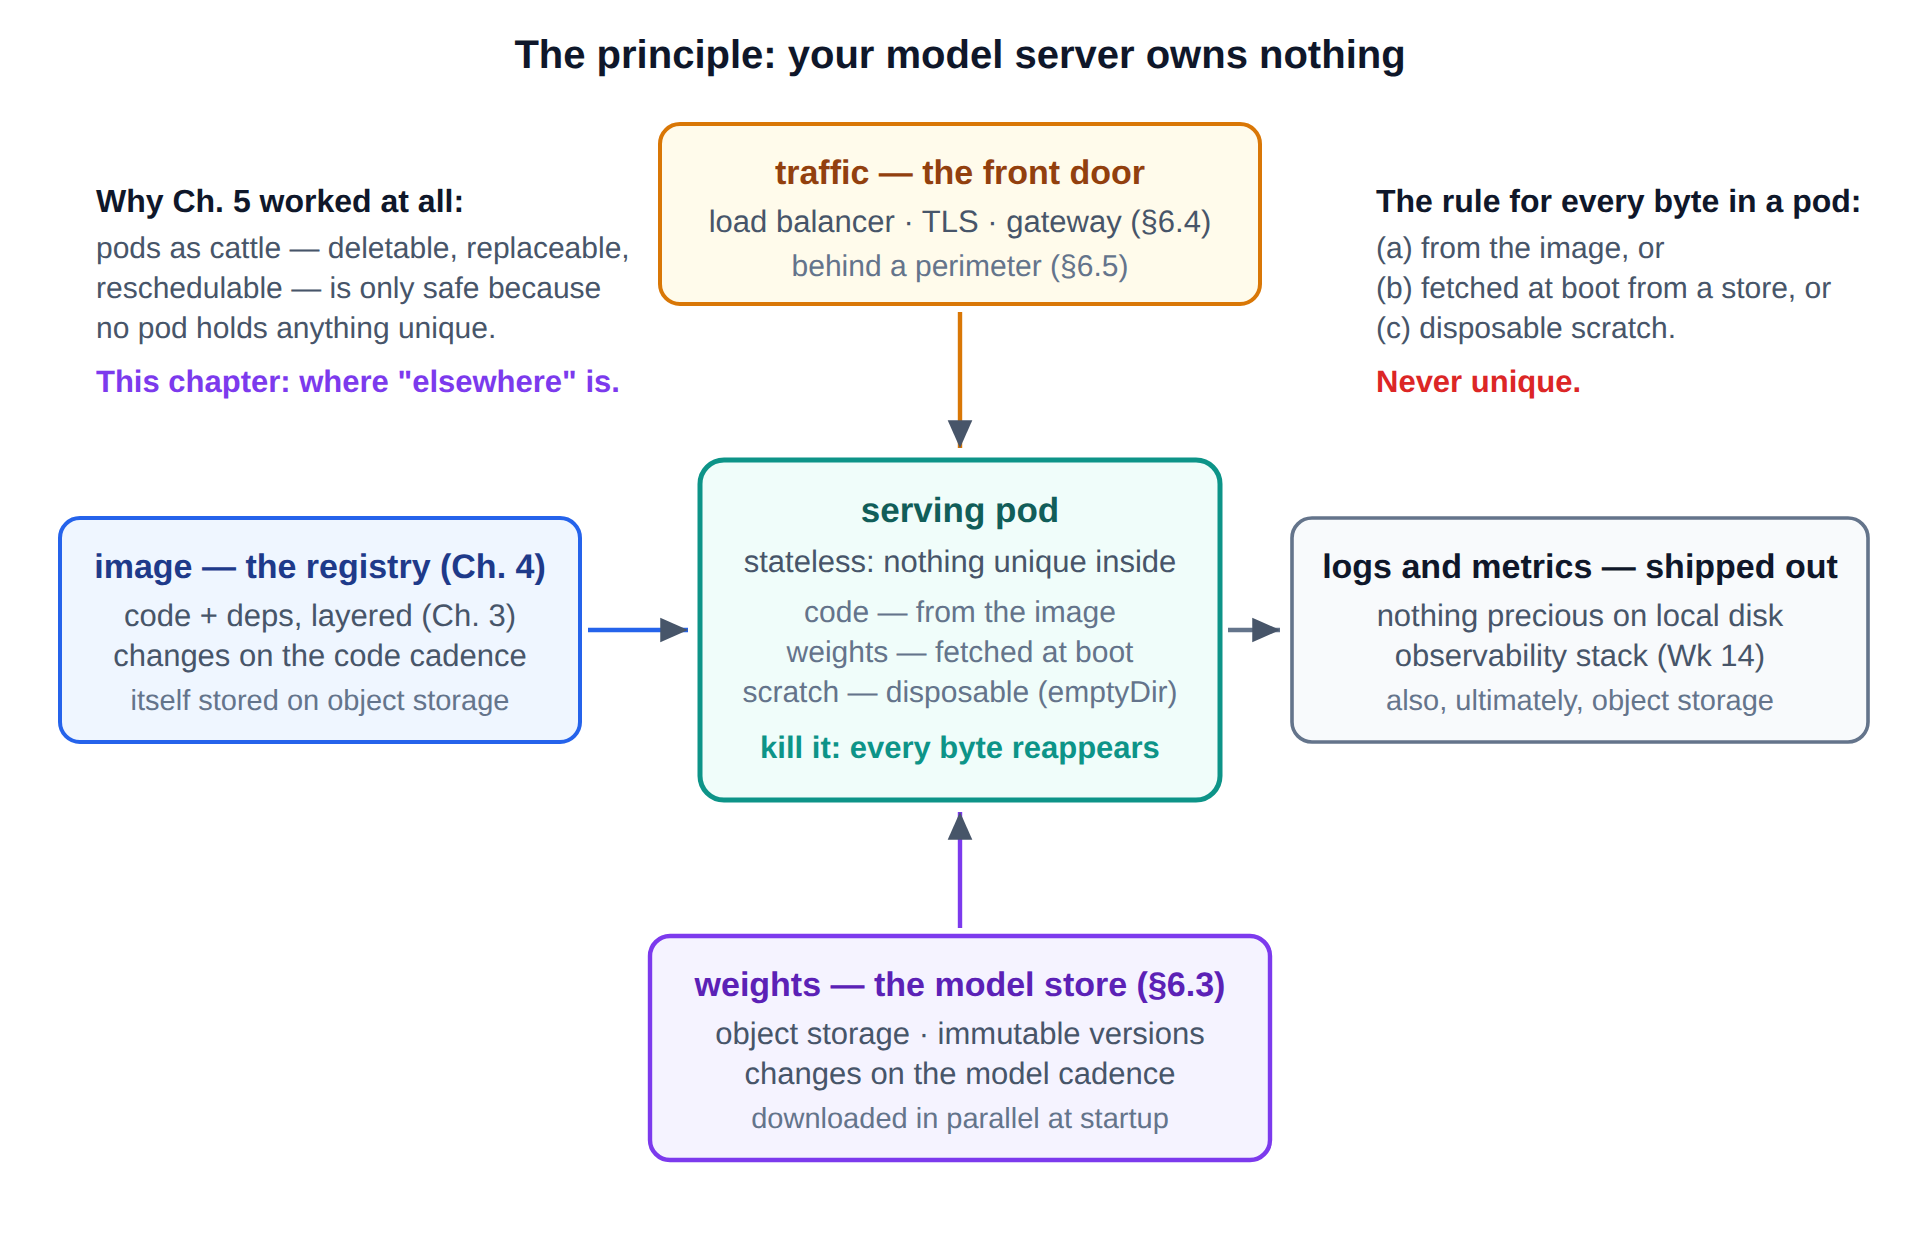
\includegraphics{figures/fig6-1_ownnothing.png}}\\[3pt]
  \figcaption{그림 6-1  아무것도 소유하지 않는 원칙. 코드는 레지스트리에서, 가중치는 모델 스토어에서 오고, 트래픽은 출입구로 들어오며, 로그는 밖으로 내보낸다. 파드를 죽여도 모든 바이트가 다시 나타난다. 이 원칙이 제5장의 모든 동작을 가능하게 했다.}
\end{tbbfigure}

\subsection*{상태 목록}

"상태 없음"은 서빙 시스템에 상태가 없다는 뜻이 아니다. 오히려 상태가 넘쳐난다. \textit{서버 프로세스}가 어떤 상태도 유일하게 보유하지 않으며, 각 상태를 형태에 맞는 계약을 제공하는 저장소로 밀어낸다는 뜻이다. 한 번은 빠짐없이 정리할 가치가 있다. 이 책에서 앞으로 나올 모든 아키텍처 논의는 사실 아래 표의 한 행에 해당하기 때문이다.

\begin{tbbtablewrap}
  \begin{tabular}{@{}>{\raggedright\arraybackslash}m{\dimexpr 0.2660\tbltextwidth-2\tabcolsep\relax} >{\raggedright\arraybackslash}m{\dimexpr 0.3723\tbltextwidth-2\tabcolsep\relax} >{\raggedright\arraybackslash}m{\dimexpr 0.3617\tbltextwidth-2\tabcolsep\relax}@{}}
  \arrayrulecolor{tbbnavy}\specialrule{1pt}{0pt}{0pt}
  \rowcolor{tbbtablehead}{\centering \bfseries\color{tbbnavy}상태} & {\centering \bfseries\color{tbbnavy}저장 위치} & {\centering \bfseries\color{tbbnavy}선택 이유} \\
  \arrayrulecolor{tbbnavy}\specialrule{0.7pt}{0pt}{2pt}
  {코드 + 의존성} & {레지스트리의 이미지(제4장)} & {버전 관리, 내용 주소 지정, 노드별 캐시} \\
  \arrayrulecolor{tbbtableborder}\hline
  {\textbf{모델 가중치}} & {\textbf{모델 스토어(model store) — 객체 스토리지(§6.3)}} & {매우 크고 변경 불가능하며 버전이 있고 모든 레플리카가 읽음} \\
  \arrayrulecolor{tbbtableborder}\hline
  {요청 상태} & {별도 저장 안 함 — 요청 자체에 존재} & {상태 없는 HTTP: 어느 레플리카든 어느 요청이든 응답 가능} \\
  \arrayrulecolor{tbbtableborder}\hline
  {캐시(토크나이저, JIT, 워밍업)} & {로컬 임시 공간(emptyDir) — 버려도 됨} & {다시 만드는 비용이 저렴하며 파드의 수명과 묶을 가치가 없음} \\
  \arrayrulecolor{tbbtableborder}\hline
  {로그 · 지표 · 트레이스} & {지속해서 외부로 전송(14주 차)} & {읽기 전에 파드가 죽을 수 있음} \\
  \arrayrulecolor{tbbtableborder}\hline
  {사용자 데이터 · 특성 · 세션} & {데이터베이스와 특성 스토어} & {트랜잭션을 지원하고 변경 가능 — 블록 기반 엔진(§6.2)} \\
  \arrayrulecolor{tbbnavy}\specialrule{1pt}{2pt}{0pt}
  \end{tabular}\par
  \figcaption{표 6-1  서빙 상태별로 알맞은 위치}
\end{tbbtablewrap}

두 행은 다시 볼 가치가 있다. \textbf{요청 상태}가 없기 때문에 제5장의 Service는 "연결마다 정상 백엔드 하나"를 가볍게 고를 수 있었다. 어느 레플리카든 어느 요청에나 응답할 수 있다면 로드 밸런싱은 자유로운 선택이다. 세션 어피니티("고정 세션")가 끌리기 시작했다면 대개 상태를 서버 안으로 몰래 들여온 것이다. 그 대가로 부하가 고르지 않고, 롤아웃마다 처리 중 요청을 비우기 어려우며, 장애 대응도 나빠진다. 그래서 서빙 시스템은 어피니티를 기능이라기보다 나쁜 냄새로 본다. \textbf{캐시}는 더 미묘하다. 워밍업된 파드는 콜드 파드와 실제로 다르다. 제3장의 페이지 캐시에는 가중치가 차 있고, 커널은 JIT로 컴파일되어 있으며, 할당기도 준비되어 있다. 상태 없음은 \textit{성능}이 아니라 \textit{정확성}에 관한 원칙이다. 캐시를 잃어도 정답을 잃어서는 안 되지만, 지연 시간은 분명 나빠질 수 있다. 바로 그래서 이 장은 콜드 스타트 비용을 항목별로 계산하고(§6.3), 12주 차에는 이를 줄이는 방법을 다룬다.

\subsection*{이 장이 제 몫을 하는 이유}

\begin{tbbitemize}
  \item \textbf{가중치 문제가 곧 서빙 문제다.} 440 MB BERT는 실수에 너그럽지만 13 GB 양자화 LLM은 그렇지 않으며, 11주 차 모델은 더 크다. 가중치가 어디에 살고 얼마나 빨리 도착하며 어떻게 버전을 관리하는지가 콜드 스타트 비용(12주 차), 배포 방식(13주 차), 그리고 청구서에서 놀랄 만큼 큰 몫(§6.5의 NAT 함정)을 결정한다.
  \item \textbf{출입구가 곧 제품이다.} 제5장의 Service에는 클러스터 내부 이름만 있다. ClusterIP로는 누구에게도 비용을 청구할 수 없다. TLS, 라우팅, 할당량, 사용량 계측(§6.4)이 Deployment를 제1장 생태계의 모델 API로 바꾼다. 강의 프로젝트도 바로 이 노출을 올바르게 구현해야 한다.
  \item \textbf{경계는 선택 사항이 아니다.} GPU 플릿은 대다수 팀이 운영하는 시스템 가운데 가장 비싸고 공격하기도 쉽다. §6.5의 VPC 패턴인 공개 출입구 하나, 사설 하드웨어, 키 없는 아이덴티티가 제대로 된 아키텍처와 사고 보고서를 가른다.
  \item \textbf{이 장에서 인프라 절반을 완성한다.} 이 장이 끝나면 커널(제2–3장), 패키징(제4장), 오케스트레이션(제5장), 상태와 경계(제6장)를 갖춘다. 이 책의 파트 2에서는 이 스택 위에서 모델을 서빙하며 아래를 다시 내려다보지 않는다. 다만 디버깅할 때는 예외이므로 §6.6이 필요하다.
\end{tbbitemize}

\begin{calloutbox}{tbbpurple}{tbbpurplefill}
{\normalsize\bfseries\color{tbbpurple}생각해 보기}\par\vspace{3pt}
\begin{tbbitemize}
  \item 대부분의 "상태 없는" 서버에 숨어 있는 상태인 처리 중 요청을 찾아보자. 종료할 때 이 상태를 비우기 위해 제3장과 제5장에서 마련한 두 메커니즘은 무엇이며, 생략하면 무엇이 깨지는가?
  \item 팀원이 사용자마다 요청이 같은 레플리카에 가도록 고정 세션(sticky session)을 제안한다("KV 캐시가 워밍업 상태를 유지할 것이다"). 롤아웃, 오토스케일 축소, 노드 장애 때 치러야 할 비용을 열거한 뒤, 11주 차 LLM 세션에서 이 긴장이 실제로 다시 나타나는 지점을 살펴보자.
  \item 대신 가중치를 이미지에 구워 넣었다고 하자(제3장 §3.4의 안티패턴). 표 6-1의 이미지 행을 따라가며 조용히 깨지는 성질을 나열하자. 이제 "버전 관리"는 무엇을 뜻하고, 코드 긴급 수정의 비용은 얼마이며, 13 GB × 매주 배포할 때 레지스트리 청구서는 어떻게 되는가?
\end{tbbitemize}
\end{calloutbox}

\section{두 가지 계약: 블록과 객체}

클라우드 스토리지는 세 계열로 나뉜다. 이들을 생산적으로 비교하는 방법은 기능 목록이 아니라 서비스가 무엇을 약속하고 그 약속에 얼마를 받는지 나타내는 \textbf{계약}을 보는 것이다. 계약을 한 번 정확히 이해하면 이 책의 모든 스토리지 결정은 패턴 맞추기로 단순해진다. 접근 패턴은 무엇이고, 누가 공유하며, 어느 정도의 내구성(durability)이 필요하고, 정확히 그 조건을 파는 계약은 무엇인가(그림 6-2)?

\subsection*{블록: 연결해서 쓰는 디스크}

\textbf{블록 스토리지}(AWS EBS, GCP Persistent Disk)는 컴퓨팅에서 가장 오래된 약속인 \textit{디스크}를 판매한다. 원하는 크기의 원시 장치를 받으며 OS는 이를 로컬 하드웨어와 구별하지 못한다. 사실 제2장의 virtio 이야기가 다시 등장한 것이다. 블록은 네트워크 너머의 복제 스토리지 서버에 있지만 반가상화 디스크로 보인다. 여기에 파일 시스템을 올리면 임의 읽기·쓰기, 제자리 갱신, 바이트 단위 탐색, 밀리초 미만에서 밀리초 단위의 지연 시간까지 완전한 POSIX 의미 체계를 얻는다. 데이터베이스에 필요한 계약이 바로 이것이다. B-tree는 4,381번 페이지를 초당 만 번 제자리에서 다시 쓰고 싶어 한다. 가격도 그에 맞게 책정된다. 용량과 성능(GB 단위 크기, IOPS, 처리량)을 \textbf{프로비저닝(provisioning)}하고 실제 사용 여부와 관계없이 예약한 만큼 비용을 낸다(gp3급: 대표값 월 GB당 약 \$0.08). 운영상 중요한 작은 조항이 두 가지 있다. 블록 볼륨은 \textbf{한 번에 인스턴스 하나에만} 연결되며(공유 공간이 아니라 디스크다), \textbf{하나의 가용 영역}에 존재한다. 그 이상의 내구성은 스냅샷으로 직접 책임져야 하며, 흥미롭게도 스냅샷은 객체 스토리지에 저장된다.

\begin{terminalbox}
\begin{Verbatim}[breaklines=true,breakanywhere=true,fontsize=\small,formatcom=\color{tbbtermfg},codes=\tbbcodeactive]
$ lsblk
NAME     SIZE  TYPE  MOUNTPOINT
nvme0n1  100G  disk  /              # boot volume (also block!)
nvme1n1  200G  disk                 # the EBS volume we attached
$ sudo mkfs.ext4 /dev/nvme1n1 && sudo mount /dev/nvme1n1 /scratch
$ dd if=/dev/zero of=/scratch/t bs=4k count=1 oflag=dsync
4096 bytes copied, 0.00089 s      # ~0.9 ms: a disk-shaped latency
# the OS cannot tell this from local hardware. that is the product.
\end{Verbatim}
\end{terminalbox}
\figcaption{터미널 기록 6-2  직접 체감하는 블록 계약. 연결하고, 포맷하고, 마운트한 뒤 밀리초 미만으로 쓴다. 모든 줄 아래에서 제2장의 virtio 메커니즘이 작동한다.}

\subsection*{객체: 호출해서 쓰는 API}

\textbf{객체 스토리지}(S3, GCS)는 전혀 다른 약속, 즉 \textit{HTTP API 뒤에 놓인 내구성 높은 블롭}을 판매한다. 장치도, 파일 시스템도, 탐색도 없다. \code{bert-classifier/\allowbreak v7/\allowbreak model.safetensors} 같은 키 아래에 최대 5 TB인 객체를 \code{PUT}하고, 전체 또는 원하는 바이트 범위를 \code{GET}한다. 제자리 편집은 할 수 없다. "객체의 100–200번 바이트를 덮어쓴다"는 동작이 없으므로 객체 전체를 교체하거나 아예 건드리지 않아야 한다. 디스크 의미 체계를 포기하는 대신 디스크가 제공할 수 없는 성질을 얻는다. \textbf{내구성}은 일레븐 나인(99.999999999\%)이다. 모든 객체를 여러 장치와 가용 영역에 삭제 코딩해 달성한다. 객체 하나가 사라져도 뉴스가 될 정도이며 누구도 S3를 스냅샷하지 않는다. \textbf{규모와 공유} 측면에서는 용량이 사실상 무제한이고 리전 안의 \textit{모든} 읽기 주체가 동시에 가져갈 수 있다. 파드 천 개가 같은 가중치를 끌어오는 일도 평범한 화요일일 뿐이다. \textbf{가격}은 실제 저장량(표준 클래스 월 GB당 약 \$0.023), 요청 수(GET 1,000회당 약 \$0.0004), 그리고 모두가 잊는 조항인 \textbf{외부로 나가는 바이트 수}(인터넷 외부 전송 GB당 약 \$0.09, §6.5에서 NAT 변형을 더한다)에 따라 낸다. 지연 시간에 관한 작은 조항도 있다. \textbf{첫 바이트 도착 시간은 수십 밀리초}로 디스크보다 100배 느리지만, 이후 각 스트림은 50–100 MB/s를 내고 스트림은 병렬로 늘릴 수 있다. 많은 객체의 여러 범위를 병렬로 요청하면 객체 스토리지가 10 Gbps NIC를 기꺼이 포화시킨다. 시작은 느리지만 합계에는 사실상 상한이 없는 형태를 기억하자. §6.3 전체가 이를 활용한다.

\begin{terminalbox}
\begin{Verbatim}[breaklines=true,breakanywhere=true,fontsize=\small,formatcom=\color{tbbtermfg},codes=\tbbcodeactive]
$ aws s3 cp model.safetensors s3://ml-models/bert-classifier/v7/
upload: ./model.safetensors to s3://ml-models/.../model.safetensors
$ curl -sI "$(aws s3 presign s3://ml-models/.../model.safetensors)" \
    -H "Range: bytes=0-1048575" | grep -E "HTTP|Content-Range"
HTTP/1.1 206 Partial Content
Content-Range: bytes 0-1048575/461301120
# a ranged GET: any slice of any object, over plain HTTPS.
# no mount, no filesystem, no single owner - and 206 is the
# status code your parallel loader (sec. 6.3) lives on.
\end{Verbatim}
\end{terminalbox}
\figcaption{터미널 기록 6-3  직접 체감하는 객체 계약. 업로드는 HTTP PUT이고 사전 서명 URL과 Range 헤더를 사용하면 440 MB 객체의 원하는 1 MB를 가져올 수 있다. 병렬 처리는 이 요청을 여러 개 보내는 것뿐이다.}

두 조항을 더하면 계약이 완성된다. \textbf{일관성}: S3는 2020년부터 강한 일관성을 제공한다. \code{PUT} 뒤의 \code{GET}은 새 객체를 반환하며 예외가 없다. 덕분에 10년간 전승되던 우회책이 사라졌다. 따라서 §6.3에서 세울 규율인 변경 불가능한 버전은 일관성 버그가 아니라 \textit{운영}의 제정신을 지키기 위한 것이다. \textbf{계층}: 같은 API 뒤에 저장 가격은 낮아지고 검색 비용은 높아지는 여러 \textbf{스토리지 클래스}(표준 → 비정기 접근 → 아카이브)가 있으며, \textbf{수명 주기 규칙}이 객체 나이에 따라 계층 사이를 이동시킨다. 모델 스토어에서는 플릿 규모에서 중요하다. 작년의 모델 버전 400개에 표준 클래스 가격을 낼 필요는 없다. "현재 버전이 아니면 30일 뒤 비정기 접근으로 이동" 같은 한 줄짜리 수명 주기 규칙이 깔끔한 청구서와 계속 불어나는 청구서를 가른다.

\subsection*{파일, PersistentVolumes, 그리고 솔직한 비교표}

세 번째 계열인 \textbf{파일 스토리지(file storage)}(서비스형 NFS: EFS, Filestore)는 절충 계약이다. 블록보다 GB당 약 네 배 비싼 가격과 네트워크 파일 시스템 지연 시간을 감수하고 POSIX 의미 체계와 많은 동시 읽기·쓰기 주체를 함께 얻는다. 여러 학습 작업이 이어 쓰는 공유 캐시처럼 여러 파드가 \textit{변경 가능한} 파일을 공유해야 할 때 제값을 한다. 하지만 객체 스토어와 로컬 캐시의 조합이 더 저렴하고 빠른 곳에서도 흔히 잘못 구매한다. Kubernetes에서 블록과 파일은 \textbf{PersistentVolume}으로 드러난다. \code{ReadWriteOnce}(RWO) 접근을 사용하는 PVC는 한 번에 노드 하나만 쓸 수 있는, 정확히 디스크 계약인 블록이다. \code{ReadWriteMany}(RWX)는 파일이다. 의미심장하게도 객체 스토리지는 이 목록에 아예 없다. 마운트하는 볼륨이 아니라 호출하는 API이기 때문에 파일 시스템의 방해 없이 읽기 주체 천 개가 공유할 수 있다. (버킷을 파일 시스템으로 마운트하는 s3fs, mountpoint 같은 FUSE 어댑터도 있으며 탐색에는 편리하다. 다만 편의용 연결 계층으로만 보고, 객체 스토리지에 애초에 하지 않은 디스크 약속을 지키게 하는 수단으로 여겨서는 안 된다.)

\begin{tbbtablewrap}
  \begin{tabular}{@{}>{\raggedright\arraybackslash}m{\dimexpr 0.2181\tbltextwidth-2\tabcolsep\relax} >{\raggedright\arraybackslash}m{\dimexpr 0.2660\tbltextwidth-2\tabcolsep\relax} >{\raggedright\arraybackslash}m{\dimexpr 0.2766\tbltextwidth-2\tabcolsep\relax} >{\raggedright\arraybackslash}m{\dimexpr 0.2394\tbltextwidth-2\tabcolsep\relax}@{}}
  \arrayrulecolor{tbbnavy}\specialrule{1pt}{0pt}{0pt}
  \rowcolor{tbbtablehead}{\centering \bfseries\color{tbbnavy}} & {\centering \bfseries\color{tbbnavy}블록(EBS)} & {\centering \bfseries\color{tbbnavy}객체(S3)} & {\centering \bfseries\color{tbbnavy}파일(EFS)} \\
  \arrayrulecolor{tbbnavy}\specialrule{0.7pt}{0pt}{2pt}
  {\textbf{제공 형태}} & {원시 디스크} & {블롭을 다루는 HTTP API} & {공유 POSIX 트리} \\
  \arrayrulecolor{tbbtableborder}\hline
  {\textbf{의미 체계}} & {제자리 임의 읽기·쓰기} & {전체 또는 범위 PUT/GET, 편집 불가} & {POSIX, 동시 접근} \\
  \arrayrulecolor{tbbtableborder}\hline
  {\textbf{지연 시간}} & {밀리초 미만–밀리초} & {첫 바이트까지 수십 밀리초} & {밀리초(네트워크 홉)} \\
  \arrayrulecolor{tbbtableborder}\hline
  {\textbf{처리량}} & {볼륨별 프로비저닝} & {\textbf{병렬: NIC 포화까지}} & {프로비저닝·버스트} \\
  \arrayrulecolor{tbbtableborder}\hline
  {\textbf{공유}} & {인스턴스 하나(RWO)} & {읽기 주체 제한 없음} & {다수 읽기·쓰기(RWX)} \\
  \arrayrulecolor{tbbtableborder}\hline
  {\textbf{내구성}} & {AZ 하나 + 직접 만든 스냅샷} & {\textbf{일레븐 나인(eleven nines), AZ 간 복제}} & {다중 AZ, 관리형} \\
  \arrayrulecolor{tbbtableborder}\hline
  {\textbf{가격 형태}} & {프로비저닝한 용량: 월 GB당 약 \$0.08} & {월 GB당 약 \$0.023 + 요청 + 외부 전송} & {사용량: 월 GB당 약 \$0.30} \\
  \arrayrulecolor{tbbtableborder}\hline
  {\textbf{서빙 용도}} & {데이터베이스 · 노드 임시 공간} & {\textbf{가중치 · 데이터셋 · 이미지 · 로그}} & {공유 변경 가능 캐시} \\
  \arrayrulecolor{tbbnavy}\specialrule{1pt}{2pt}{0pt}
  \end{tabular}\par
  \figcaption{표 6-2  세 가지 계약 비교(대표 가격)}
\end{tbbtablewrap}

\begin{calloutbox}{tbbblue}{tbbbluefill}
{\normalsize\bfseries\color{tbbblue}계산 예시 — 하나의 13 GB 모델을 저장하는 네 가지 방법}\par\vspace{3pt}
13 GB 모델을 노드 5개에 걸친 레플리카 20개에서 사용할 수 있어야 한다. 월 스토리지 비용과 동작을 비교해 보자(대표 가격).

\begin{tbbitemize}
  \item \textbf{객체 스토어(권장 패턴):} 복사본 하나에 13 GB × \$0.023 ≈ \textbf{월 \$0.30}이며, 배포마다 GET 요청 비용이 몇 센트 더 든다. 각 노드는 처음 가져올 때 이미 있는 블록 임시 공간에 로컬 캐시한다. 버전 관리는 새 접두사를 만드는 것으로 거의 무료다.
  \item \textbf{노드별 블록 볼륨:} 5 × 13 GB × \$0.08 ≈ \textbf{월 \$5.20}에 더해 새 버전을 디스크 5개에 원자적으로 배포하고 롤백하는 오케스트레이션까지 직접 책임져야 한다. 더 나쁜 모델 스토어를 다시 만든 셈이다.
  \item \textbf{파일 공유:} 13 GB × \$0.30 ≈ \textbf{월 \$3.90}이며 공유 마운트라 간편하다. 다만 레플리카 20개가 동시에 콜드 스타트해 하나의 공유 처리량을 두고 경합할 때까지다. 버전 관리 규율도 여전히 필요하다.
  \item \textbf{이미지에 구워 넣기(제3장의 안티패턴):} 레지스트리도 어차피 객체 스토리지 위에 있으므로 저장 비용은 저렴하다. 하지만 코드를 배포할 때마다 레지스트리 경로를 통해 13 GB × 노드 5개를 다시 보내고, 모델 버전이 이미지 버전에 용접된다. 실제 비용은 GB가 아니라 워크플로다.
\end{tbbitemize}

승리하는 패턴은 \textbf{객체 스토어를 원본으로, 블록을 노드별 캐시로} 쓰는 조합이다. 한 번 저장하고 로컬에 캐시하며 접두사로 버전을 관리한다. 이 조합에는 이름이 있으며 다음 절에서 다룬다.
\end{calloutbox}

\vspace{3.0pt}

\begin{tbbfigure}
  \adjustbox{max width=0.94\linewidth,max totalheight=0.46\textheight}{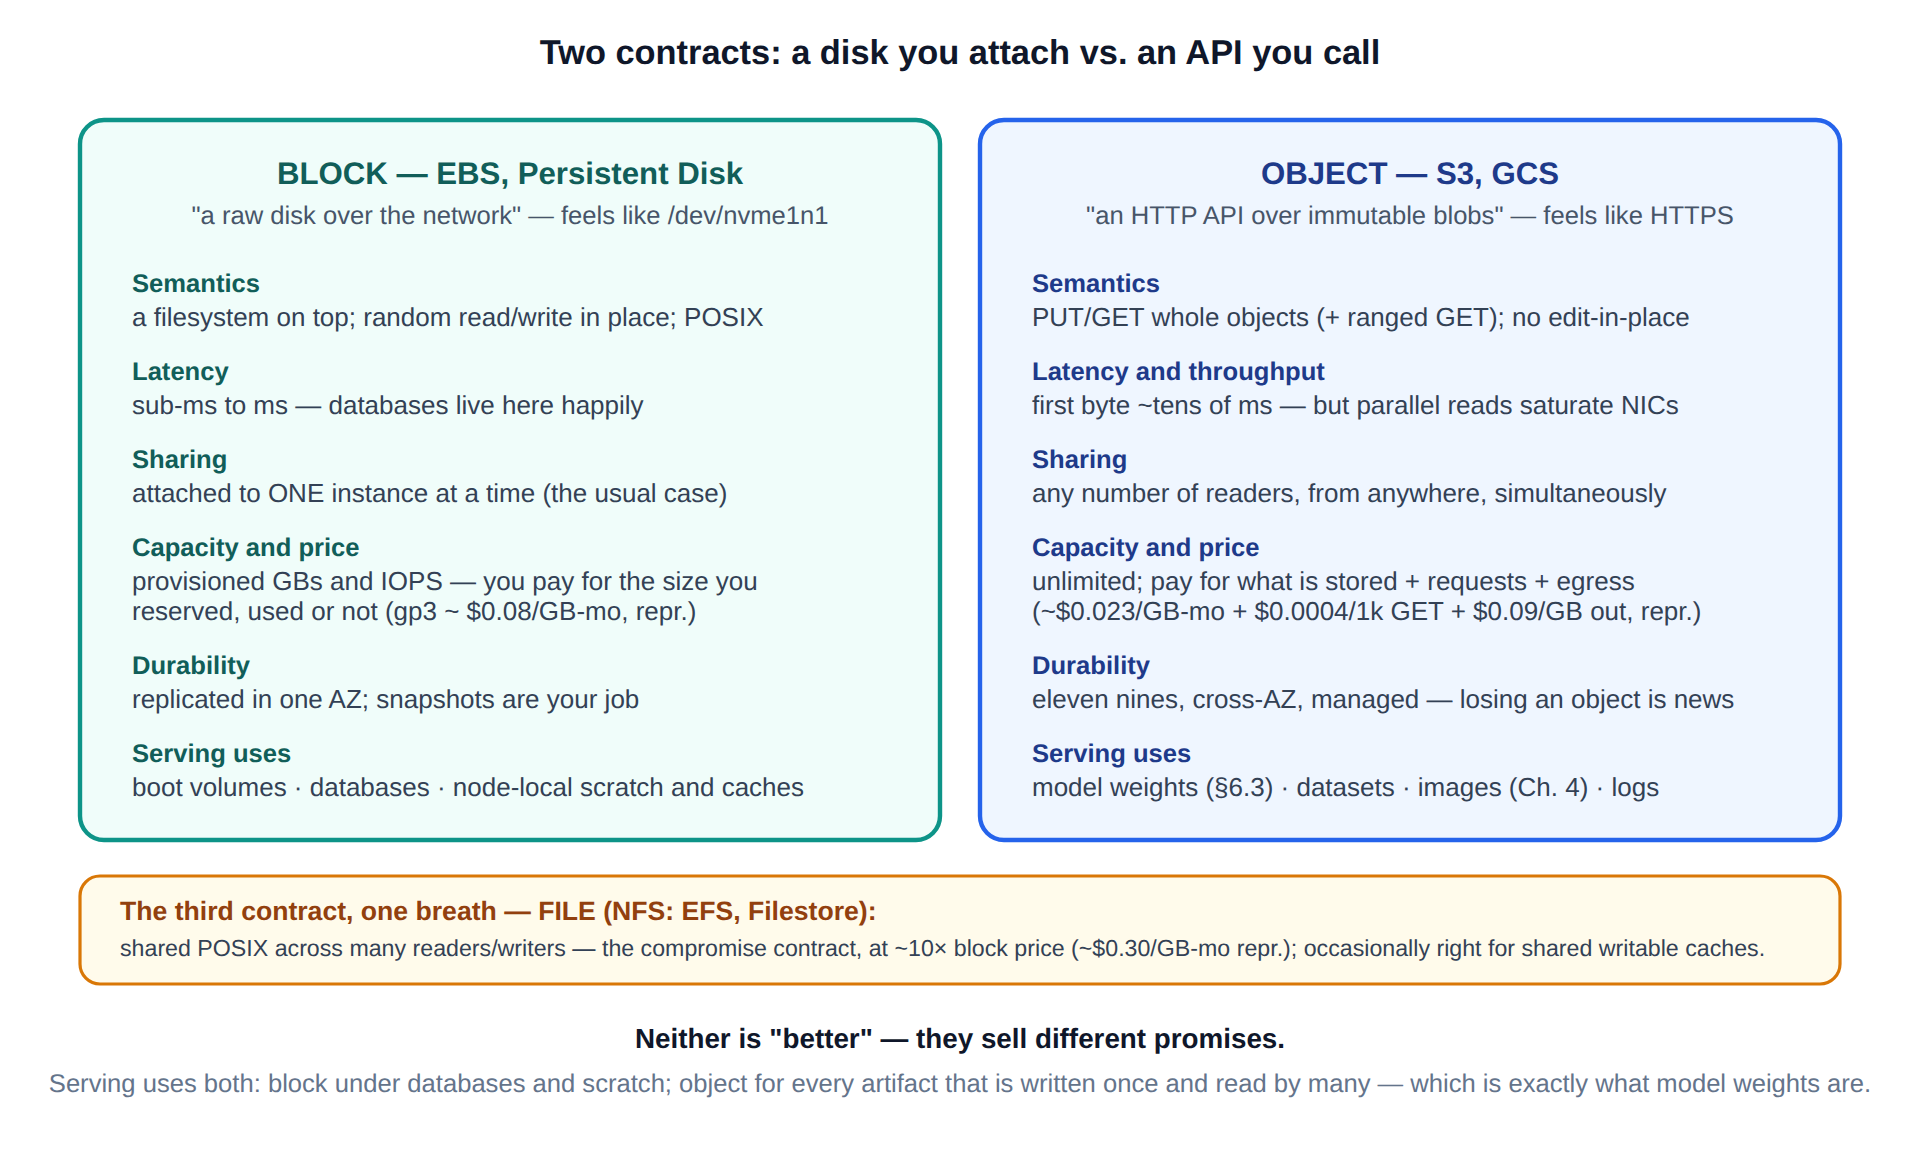
\includegraphics{figures/fig6-2_contracts.png}}\\[3pt]
  \figcaption{그림 6-2  두 가지 계약. 블록은 디스크(POSIX, 마이크로초 단위, 소유자 하나)를 팔고, 객체는 HTTP 뒤의 내구성 높은 블롭(범위 읽기, 제한 없는 읽기 주체, 병렬 처리량)을 판다. 파일은 비싼 절충안이다.}
\end{tbbfigure}

\begin{calloutbox}{tbbpurple}{tbbpurplefill}
{\normalsize\bfseries\color{tbbpurple}생각해 보기}\par\vspace{3pt}
\begin{tbbitemize}
  \item PostgreSQL 데이터베이스를 객체 스토리지에서 실행하는 것은 끔찍한 생각이지만 분석 엔진은 하루 종일 S3의 Parquet 파일을 즐겁게 질의한다. 두 워크로드 사이에서 무엇이 달라졌는가? 이를 결정하는 계약 조항 두 가지를 말하자.
  \item S3는 일레븐 나인의 내구성을 약속하지만 가용성 SLA는 약 99.9\%로 훨씬 낮다. 둘의 차이는 무엇이며, 이 간격 때문에 로더(§6.3)는 무엇을 해야 하는가?
  \item 팀이 "현재 모델"을 보관하는 RWX 파일 공유 하나를 두고, 출시 때마다 제자리에서 업데이트하려 한다. 데모에서는 동작한다. 한 분기 안에 문제를 일으킬 세 가지 방식을 나열하자. 다운로드 중 갱신, 롤백, 콜드 스타트 경합을 생각해 보자.
\end{tbbitemize}
\end{calloutbox}

\section{모델 스토어}

제3장 §3.4는 \textit{"모델 가중치는 보통 이미지 레이어에 둘 것이 아니라 모델 스토어에 보관하고 시작할 때 로딩해야 한다"}는 약속을 남기며 끝났다. 이 절에서 그 약속을 지킨다. 논리는 워크로드와 계약이 완벽하게 맞는다는 데 있다. 가중치는 \textbf{매우 크고}(수백 MB에서 수백 GB), \textbf{변경 불가능하며}(학습된 산출물은 바뀌지 않고 새 학습은 새 산출물이다), \textbf{버전이 있고}(여러 버전을 보관하고 전환한다), \textbf{한 번 쓰고 모든 레플리카가 읽으며}, 병렬화하기 좋은 \textbf{대규모 순차 읽기}로 소비된다. §6.2의 객체 계약을 다시 읽어 보면 정확히 같은 목록이다. 가중치는 시스템 전체에서 가장 객체다운 바이트다(그림 6-3).

\begin{tbbfigure}
  \adjustbox{max width=0.94\linewidth,max totalheight=0.46\textheight}{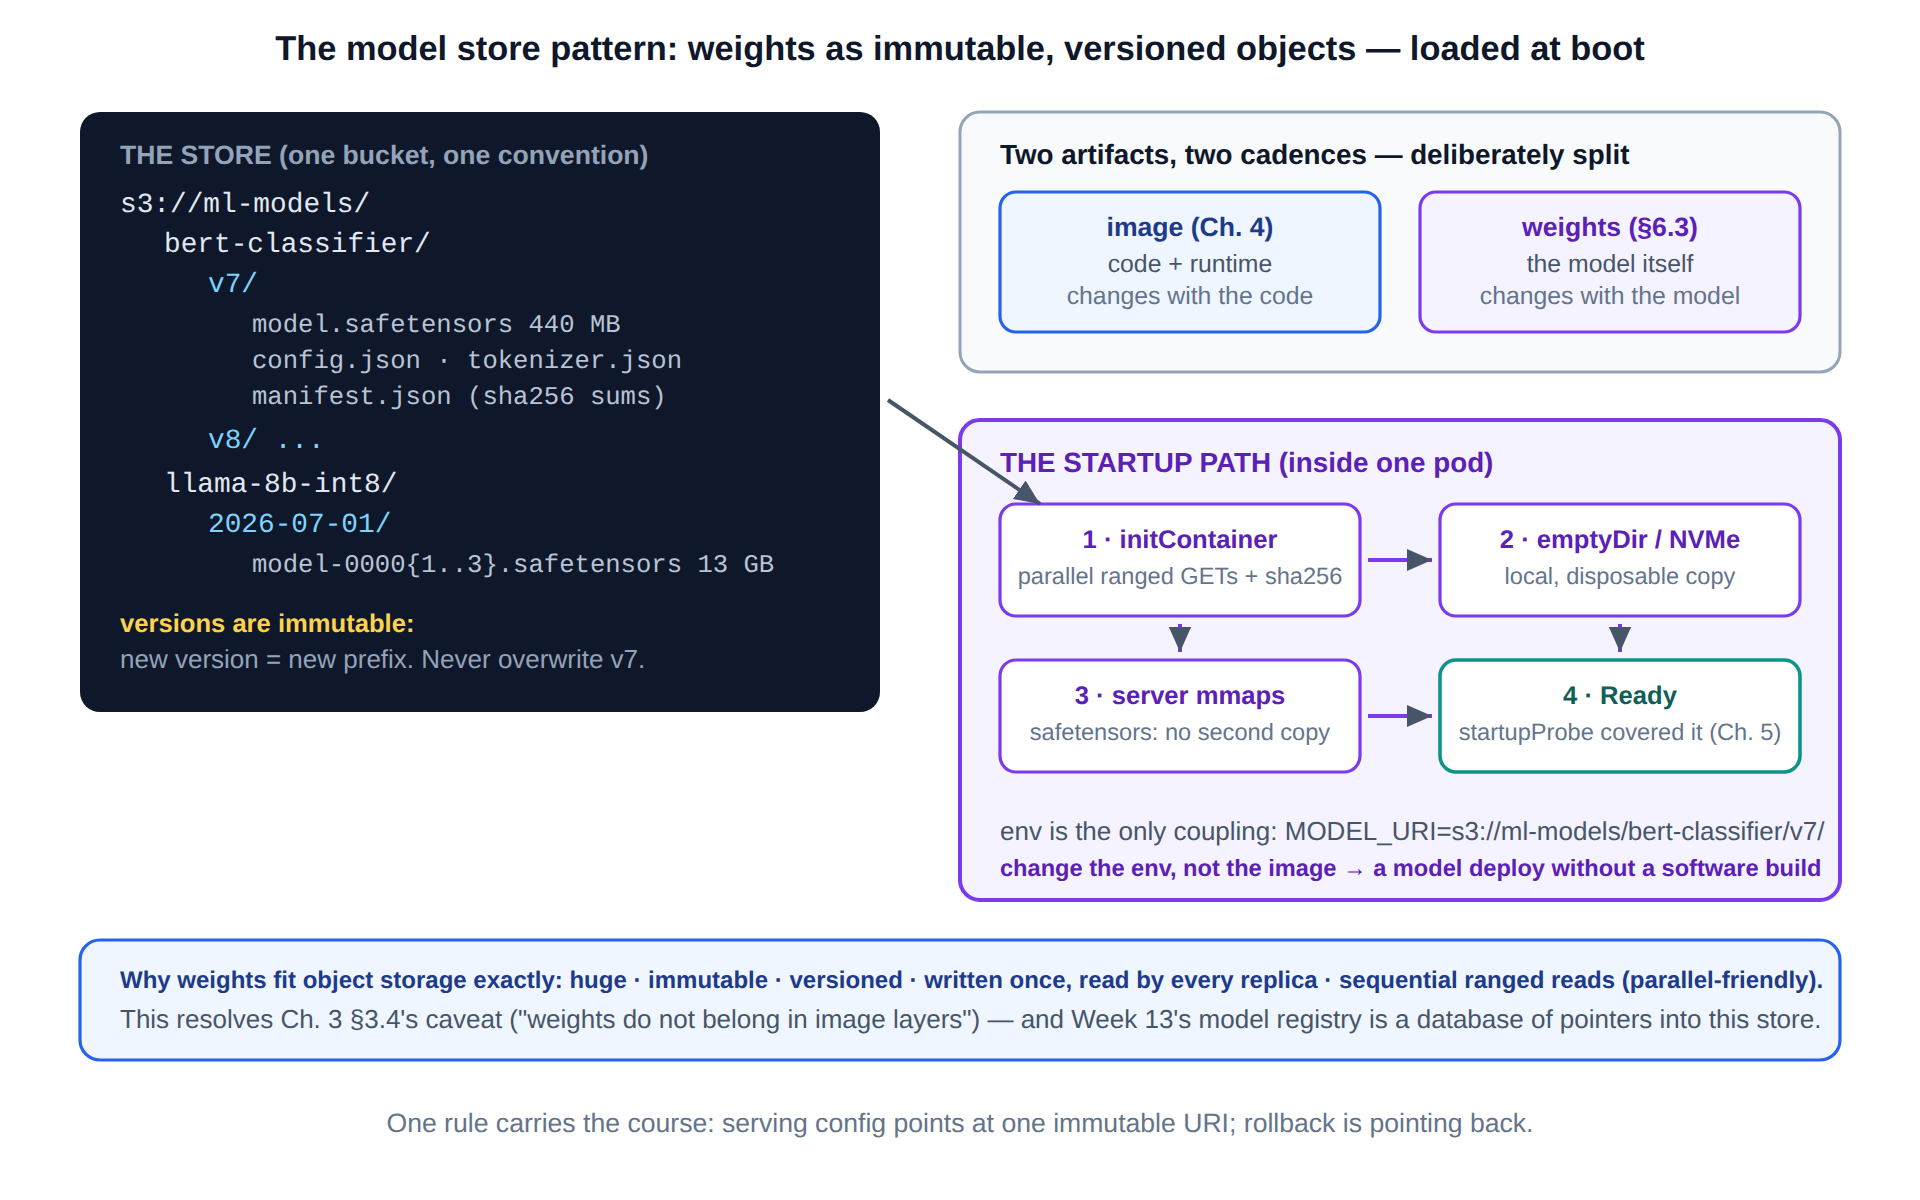
\includegraphics{figures/fig6-3_modelstore.png}}\\[3pt]
  \figcaption{그림 6-3  모델 스토어. 버킷 하나, 이름 규칙 하나, 변경 불가능한 버전, 그리고 URI를 서빙 모델로 바꾸는 시작 경로로 구성된다. 환경 변수가 이미지와 가중치 사이의 유일한 결합 지점이다.}
\end{tbbfigure}

\subsection*{레이아웃: 하나의 규칙과 변경 불가능성}

\begin{terminalbox}
\begin{Verbatim}[breaklines=true,breakanywhere=true,fontsize=\small,formatcom=\color{tbbtermfg},codes=\tbbcodeactive]
$ aws s3 ls s3://ml-models/ --recursive --human-readable | head -12
bert-classifier/v7/model.safetensors        440.0 MiB
bert-classifier/v7/config.json                1.2 KiB
bert-classifier/v7/tokenizer.json           695.4 KiB
bert-classifier/v7/manifest.json              0.6 KiB
bert-classifier/v8/model.safetensors        440.1 MiB
bert-classifier/v8/...
llama-8b-int8/2026-07-01/model-00001.safetensors  4.9 GiB
llama-8b-int8/2026-07-01/model-00002.safetensors  4.9 GiB
llama-8b-int8/2026-07-01/model-00003.safetensors  3.4 GiB
llama-8b-int8/2026-07-01/manifest.json            0.7 KiB
$ cat manifest.json   # (from v7)
{ "model": "bert-classifier", "version": "v7",
  "files": { "model.safetensors":
    "sha256:9f2c4a01..." },
  "trained": "2026-06-14", "framework": "torch-2.6" }
\end{Verbatim}
\end{terminalbox}
\figcaption{터미널 기록 6-4  스토어의 전체 스키마. 모델·버전·파일과 모든 다운로드를 검증할 수 있게 하는 sha256 합계가 든 매니페스트다. 제4장의 내용 주소 지정 이미지 레이어와 의도적으로 운을 맞췄다.}

배치는 민망할 만큼 단순한 \code{<model>/\allowbreak <version>/\allowbreak <files>}이며, 전체 패턴은 한 가지 규율에 기대어 있다. \textbf{버전은 변경할 수 없다.} 새 학습 실행, 새 양자화, 토크나이저(tokenizer) 파일 수정까지 모두 새 접두사를 사용한다. 아무리 마감이 급해도 \code{v7/\allowbreak }을 제자리에서 덮어써서는 안 된다. 이유는 계속 쌓인다. 롤링 업데이트(제5장)에서는 몇 분 동안 기존 파드와 새 파드가 나란히 실행된다. 그 아래의 \code{v7}이 바뀔 수 있으면 \textit{선언한 버전이 같은} 레플리카끼리도 서로 다른 결과를 낸다. 아래에서 볼 노드 캐시는 URI를 키로 사용하므로 내용을 바꾸면 모든 캐시가 조용히 오염된다. 롤백(제5장의 \code{rollout undo}, 13주 차 자동화)은 돌아갈 대상이 변경되지 않은 채 그대로 존재할 때만 의미가 있다. \code{manifest.json}의 체크섬은 모든 소비자가 다운로드를 스스로 검증하게 한다. 제4장의 이미지 다이제스트에 적용한 무결성 아이디어를 스택에서 한 단계 위의 산출물에 적용한 것이다. 변경 불가능성은 "어느 모델이 실행 중인가?"라는 질문을 조사 작업에서 문자열 비교로 바꾼다. URI \textit{자체}가 답이다.

\subsection*{빠르게 로딩하기: 병렬 로더}

이제 성능 측면을 보자. 첫 바이트는 느리지만 합계에는 사실상 상한이 없다는 객체 계약의 형태를 떠올리고, 순진한 로더의 동작을 살펴보자. \code{GET} 하나, 스트림 하나로 운이 좋아야 약 80 MB/s다. 13 GB라면 GPU 노드가 비용만 내며 아무 일도 하지 않는 \textbf{162초}다. 해결책은 \textit{계약을 활용하는 것}이다. 객체를 여러 범위로 나누고 8–16개 범위를 동시에 가져와(터미널 기록 6-3의 \code{206 Partial Content}를 여러 번 실행) 제자리에 쓴다. 총 처리량은 \textbf{NIC}(10 Gbps ≈ 1.25 GB/s 상한)나 로컬 디스크에 닿을 때까지 증가한다. 이 규모에서는 S3 자체가 병목이 되지 않으며 접두사마다 대규모 요청 병렬 처리를 명시적으로 지원한다. 전용 도구인 \code{s5cmd}, 동시성을 설정할 수 있는 AWS CLI, \code{hf\_transfer}도 정확히 이 방식을 구현한다. 실습에서는 최소한의 로더를 직접 작성해 메커니즘을 익힌다.

\begin{terminalbox}
\begin{Verbatim}[breaklines=true,breakanywhere=true,fontsize=\small,formatcom=\color{tbbtermfg},codes=\tbbcodeactive]
# the experiment the lab reproduces (13 GB, same node, same bucket):
$ time python loader.py --streams 1 $MODEL_URI /models
real  2m42.1s                       # ~80 MB/s: one stream
$ time python loader.py --streams 16 $MODEL_URI /models
real  0m16.8s                       # ~790 MB/s: sixteen ranged streams
# 9.6x from the same bucket, same NIC - the contract, exploited.
$ sha256sum -c <(python manifest_sums.py /models/manifest.json)
model-00001.safetensors: OK
model-00002.safetensors: OK
model-00003.safetensors: OK        # verify before you serve. always.
\end{Verbatim}
\end{terminalbox}
\figcaption{터미널 기록 6-5  병렬 로더. 하나의 GET을 16개의 범위 GET으로 바꿔 162 s → 17 s로 줄인 뒤, 첫 요청을 서빙하기 전에 매니페스트를 기준으로 체크섬을 검증한다.}

다운로드 다음에는 \textbf{로드}가 오며, 형식을 하나 잘 고르면 비용이 거의 사라진다. 바로 \textbf{safetensors}다. JSON 헤더(텐서 이름, 자료형, 형상, 오프셋) 뒤에 원시 텐서 바이트가 이어지는 형식이다. 로더가 역직렬화하지 않고 파일을 \code{mmap}해 텐서를 무복사(zero-copy)로 \textit{제자리에서} 쓰도록 설계된 형식이다. pickle 기반 체크포인트와 달리 열어도 코드가 실행될 수 없다는 점은 7주 차 형식 논의의 보안 측면이다. 제3장과 연결되는 결과가 인상적이다. mmap한 가중치 파일은 \textbf{파일 기반 페이지 캐시}다. 커널은 텐서를 처음 건드릴 때 페이지를 들이고 압박이 생기면 회수할 수 있다. 정상 모델 서버의 \code{memory.current}는 제한에 가깝지만 \code{anon}은 적당히 유지되는 이유다. 이제 §3.3의 대시보드 교훈에 직접 설계한 원인이 생겼다. GPU 서빙에서는 호스트 페이지를 VRAM으로 복사하는 단계가 이어지며, 10주 차 최적화 장이 그 지점부터 시작한다.

\subsection*{파드에 연결하기: initContainer, emptyDir, 계산된 프로브}

\begin{terminalbox}
\begin{Verbatim}[breaklines=true,breakanywhere=true,fontsize=\small,formatcom=\color{tbbtermfg},codes=\tbbcodeactive]
    spec:
      volumes:
      - name: models
        emptyDir: {}              # node-local scratch; dies with pod
      initContainers:
      - name: fetch-model
        image: registry.example.com/team/model-loader:v3
        args: ["$(MODEL_URI)", "/models", "--streams", "16"]
        env:
        - { name: MODEL_URI,
            value: "s3://ml-models/bert-classifier/v7/" }
        volumeMounts: [ { name: models, mountPath: /models } ]
      containers:
      - name: server
        image: registry.example.com/team/model-server:v12
        env:
        - { name: MODEL_DIR, value: "/models" }
        volumeMounts: [ { name: models, mountPath: /models } ]
        startupProbe:             # budget = download + load + margin
          httpGet: { path: /healthz, port: 8000 }
          periodSeconds: 5
          failureThreshold: 24    # 24 x 5s = 2 min for the 440 MB case
\end{Verbatim}
\end{terminalbox}
\figcaption{터미널 기록 6-6  연결 방식. 서버가 시작되기 전에 initContainer가 emptyDir에 다운로드한다. 이제 startupProbe 예산(제5장)은 터미널 기록 6-5의 측정값으로 계산하는 숫자다.}

각 요소는 의도된 역할 하나씩을 맡는다. \textbf{initContainer}는 서버 컨테이너가 시작되기 \textit{전에} 완료될 때까지 실행된다. 따라서 서버 이미지는 로더 의존성에서 자유롭고, 다운로드 실패는 별도의 \code{Init:Error} 상태로 나타나며(제5장의 현장 안내서에서 명확히 구별 가능), 로더도 독립적으로 업그레이드할 수 있다. \textbf{emptyDir}은 정직한 임시 공간이다. 노드 디스크에서 파드와 정확히 같은 기간만 존재하며(tmpfs가 필요하면 \code{medium: Memory}), 파드와 함께 삭제되는 것은 버그가 아니라 플랫폼이 아무것도 소유하지 않는 원칙을 강제한 결과다. \textbf{startupProbe} 예산은 더 이상 구전 지식이 아니라 산술이다. 측정한 다운로드(17 s) + 로드(10 s) + 여유분 → 임계값으로 정한다. 그리고 \textbf{환경 변수가 유일한 결합 지점}이다. 서버는 \code{/\allowbreak models}를 읽고 initContainer는 \code{MODEL\_URI}에서 파일을 가져와 채운다. \textit{두 이미지 어디에도 모델 버전은 나오지 않는다.} 이제 이 장에서 가장 멋진 터미널 기록을 볼 준비가 되었다.

\begin{terminalbox}
\begin{Verbatim}[breaklines=true,breakanywhere=true,fontsize=\small,formatcom=\color{tbbtermfg},codes=\tbbcodeactive]
$ kubectl set env deploy/model-server MODEL_URI=s3://ml-models/bert-classifier/v8/
deployment.apps/model-server env updated
$ kubectl rollout status deploy/model-server && kubectl get pods \
    -o custom-columns=NAME:.metadata.name,IMAGE:.spec.containers[0].image
deployment "model-server" successfully rolled out
NAME                            IMAGE
model-server-59d8c7f9b6-2xk4p   registry.example.com/team/model-server:v12
model-server-59d8c7f9b6-m7qvw   registry.example.com/team/model-server:v12
model-server-59d8c7f9b6-tt8zn   registry.example.com/team/model-server:v12
# same image. new model. a rolling, health-gated, rollback-able
# model deploy (Ch. 5 machinery) - and no software was built.
\end{Verbatim}
\end{terminalbox}
\figcaption{터미널 기록 6-7  결실. 이제 모델 배포는 환경 변수 변경이다. IMAGE 열은 그대로 둔 채 제5장의 다른 롤아웃처럼 여분 레플리카를 만들고 준비 상태로 제어하며 되돌릴 수 있다. 13주 차에는 바로 이 한 줄을 자동화한다.}

방금 일어난 일을 잠시 되새겨 보자. 이 장 전체의 아키텍처 핵심이기 때문이다. 두 출시 주기를, 즉 코드는 이미지에 두고 가중치는 스토어에 두는 방식으로 분리하자 \textbf{모델 출시가 소프트웨어 출시이기를 멈췄다.} Dockerfile도, CI 빌드도, 레지스트리 푸시도 없다. "배포"는 필드 하나를 바꾸는 일이며, 제5장에서 만든 모든 안전 메커니즘(여분 레플리카, 준비 상태를 통한 속도 조절, 실패 시 중단, 한 명령으로 롤백)이 그대로 적용된다. 이것 \textit{자체가} 제5장의 롤아웃이기 때문이다. 13주 차 모델 레지스트리는 어느 URI가 "스테이징"이고 어느 것이 "프로덕션"인지, 누가 언제 승격했는지를 형식적으로 기록한다. 하지만 레지스트리는 메타데이터일 뿐이며 실제 메커니즘은 이 터미널 기록에 있다.

\subsection*{콜드 스타트 청구서와 캐싱 단계}

\begin{tbbfigure}
  \adjustbox{max width=0.94\linewidth,max totalheight=0.46\textheight}{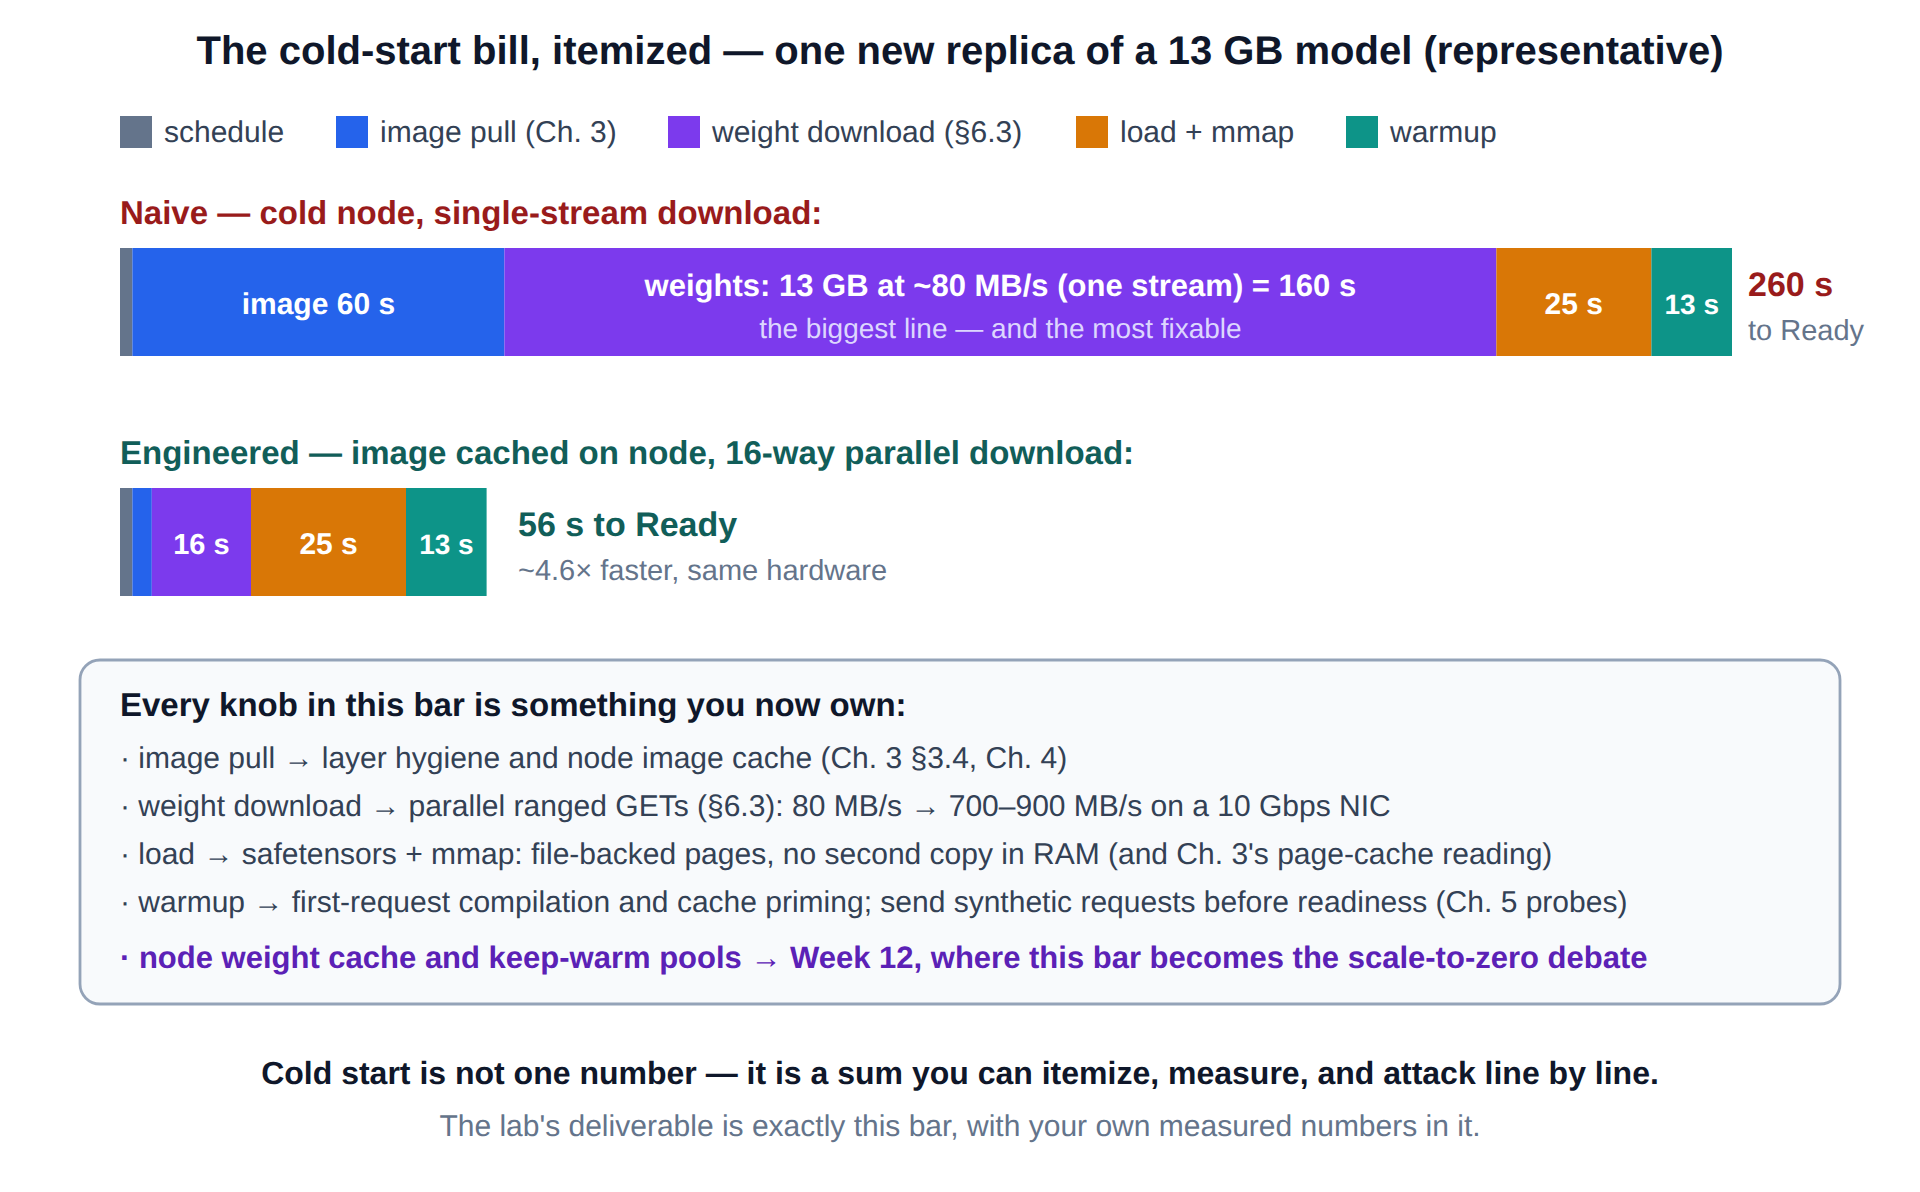
\includegraphics{figures/fig6-4_coldstart.png}}\\[3pt]
  \figcaption{그림 6-4  새 레플리카 하나의 콜드 스타트 비용을 항목별로 나눈 모습. 순진한 막대는 단일 스트림 다운로드가 지배하고, 설계한 막대는 같은 레플리카를 4.6배 빠르게 준비 상태로 만든다. 12주 차에는 이 막대를 두고 씨름한다.}
\end{tbbfigure}

\begin{calloutbox}{tbbamber}{tbbamberfill}
{\normalsize\bfseries\color{tbbamberdark}계산 예시 — 레플리카 하나의 콜드 스타트 항목별 계산(13 GB 모델)}\par\vspace{3pt}
항목을 두 번 더해 보자. 대표값이며 실습에서는 직접 측정한다.

\begin{tbbitemize}
  \item \textbf{순진한 방식:} 스케줄링 약 2 s + 이미지 가져오기 60 s(6 GB, 콜드 노드 — 제3장의 계산) + 가중치 162 s(단일 스트림) + 로드 25 s + 워밍업 13 s ≈ \textbf{준비 상태까지 260 s}다.
  \item \textbf{설계한 방식:} 스케줄링 약 2 s + 이미지 약 0 s(노드에 캐시됨) + 가중치 17 s(스트림 16개) + 로드 25 s + 워밍업 13 s ≈ \textbf{준비 상태까지 56 s}다.
\end{tbbitemize}

같은 하드웨어에서 4.6배 차이가 난다. 이제 모든 항목의 책임자를 안다. 이미지 → 레이어 위생과 노드 캐시(제3–4장), 다운로드 → 이 절의 로더, 로드 → safetensors + mmap, 워밍업 → 준비 상태 전 합성 요청(제5장의 프로브, §6.4의 상태 확인 경로)이다. 남은 수단인 파드가 공유하는 노드별 가중치 캐시, 사전 워밍업 풀(pre-warmed pool), 이 막대가 좌우하는 제로 스케일링 논의는 12주 차에서 다룬다. 그때는 이 계산을 숙지했다고 가정한다.
\end{calloutbox}

\vspace{3.0pt}

캐싱 단계를 한 문단으로 미리 살펴볼 가치가 있다. emptyDir 패턴은 \textbf{파드}마다 다시 다운로드한다. URI를 키로 사용하는 \code{hostPath}/PVC 캐시는 \textbf{노드}마다 다시 다운로드한다. 버전은 오래될 수 없고 없을 수만 있으므로 변경 불가능성이 이를 안전하게 만든다. 미리 가져오는 DaemonSet은 파드가 도착하기 \textbf{전에} 노드를 워밍업한다. 가중치를 이미지에 구워 넣는 방식은 망 분리 배포나 데모 장비 같은 정당한 \textit{극단 사례}로 남는다. 제3장에서 이미 "기본값이 아닌 결정"으로 분류했다. 각 단계는 스토리지 중복과 시작 지연 시간을 맞바꾼다. 이 책에서 반복해서 등장하며 GB 단위로 구매할 수 있는 절충 관계다.

스토어에는 마지막 거주자인 \textbf{데이터셋}도 있다. 학습 데이터, 평가 세트, 팀이 회귀 테스트에 사용할 골든 요청(golden request) 픽스처(13주 차 CI 관문)는 보통 Parquet 또는 JSONL 형식으로 같은 버킷(bucket) 규율, 즉 버전이 있는 접두사, 매니페스트, 변경 불가능성을 따른다. 서빙 경로의 지연 시간 문제를 공유하지 않으므로 새 메커니즘도 필요 없다. 스토어는 신경 쓰지 않으며 바로 그것이 핵심이다.

\begin{calloutbox}{tbbpurple}{tbbpurplefill}
{\normalsize\bfseries\color{tbbpurple}생각해 보기}\par\vspace{3pt}
\begin{tbbitemize}
  \item 당직 중 사고를 넘겨받았다. 누군가 "긴급 수정"이라며 v7의 tokenizer.json을 제자리에서 다시 업로드했고, 그 뒤 레플리카 절반이 재시작되었다. 같은 URI가 두 가지 동작을 보이는 다양한 증상을 설명하고, 캐시가 문제를 악화시키는 이유와 이를 막았을 한 줄짜리 정책을 제시하자.
  \item manifest의 sha256은 TLS가 막지 못하는 무언가를 막고, TLS는 manifest가 막지 못하는 무언가를 막는다. 두 위협을 정확히 말하자.
  \item 레플리카 100개로 확장하는 사건(12주 차)에서 모든 새 파드가 동시에 13 GB를 가져온다. (a) 파드별 emptyDir, (b) 노드 캐시, (c) 사전 워밍업 노드일 때 병목은 실제로 S3, 노드별 NIC, 노드 캐시 가운데 어디에 생기는가? 파드 4개를 실행하는 10 Gbps 노드 하나의 계산을 보여 주자.
\end{tbbitemize}
\end{calloutbox}

\section{출입구: 로드 밸런서, Ingress, 게이트웨이}

제5장의 노출 사다리는 Service에 클라우드 통로를 직접 연결하는 \code{type: LoadBalancer}에서 끝났다. 데모에는 실제로 그것만 있으면 된다. 프로덕션의 출입구에는 더 긴 목록이 필요하다. 누구도 평문으로 추론 입력을 보내지 않도록 \textbf{TLS}, 한 출입구에서 여러 서비스로 \code{/\allowbreak predict}, \code{/\allowbreak embed}, \code{staging.api.example.com}을 나누는 \textbf{라우팅}, 제1장의 모델 API 경제를 움직이는 키와 계량기를 위한 \textbf{인증과 할당량}, LB 뒤의 다른 무엇보다 긴 추론 꼬리를 감당하도록 \textbf{의도적으로 선택한 타임아웃과 재시도}, §6.6에서 상태 코드를 읽기 위한 \textbf{엣지에서의 관측 가능성}이 필요하다. 이 절에서는 로드 밸런서, Ingress, 게이트웨이라는 세 계층으로 출입구를 만든 뒤, 특히 모델 서빙을 망가뜨리는 설정을 충분히 살펴본다(그림 6-5).

\begin{tbbfigure}
  \adjustbox{max width=0.94\linewidth,max totalheight=0.46\textheight}{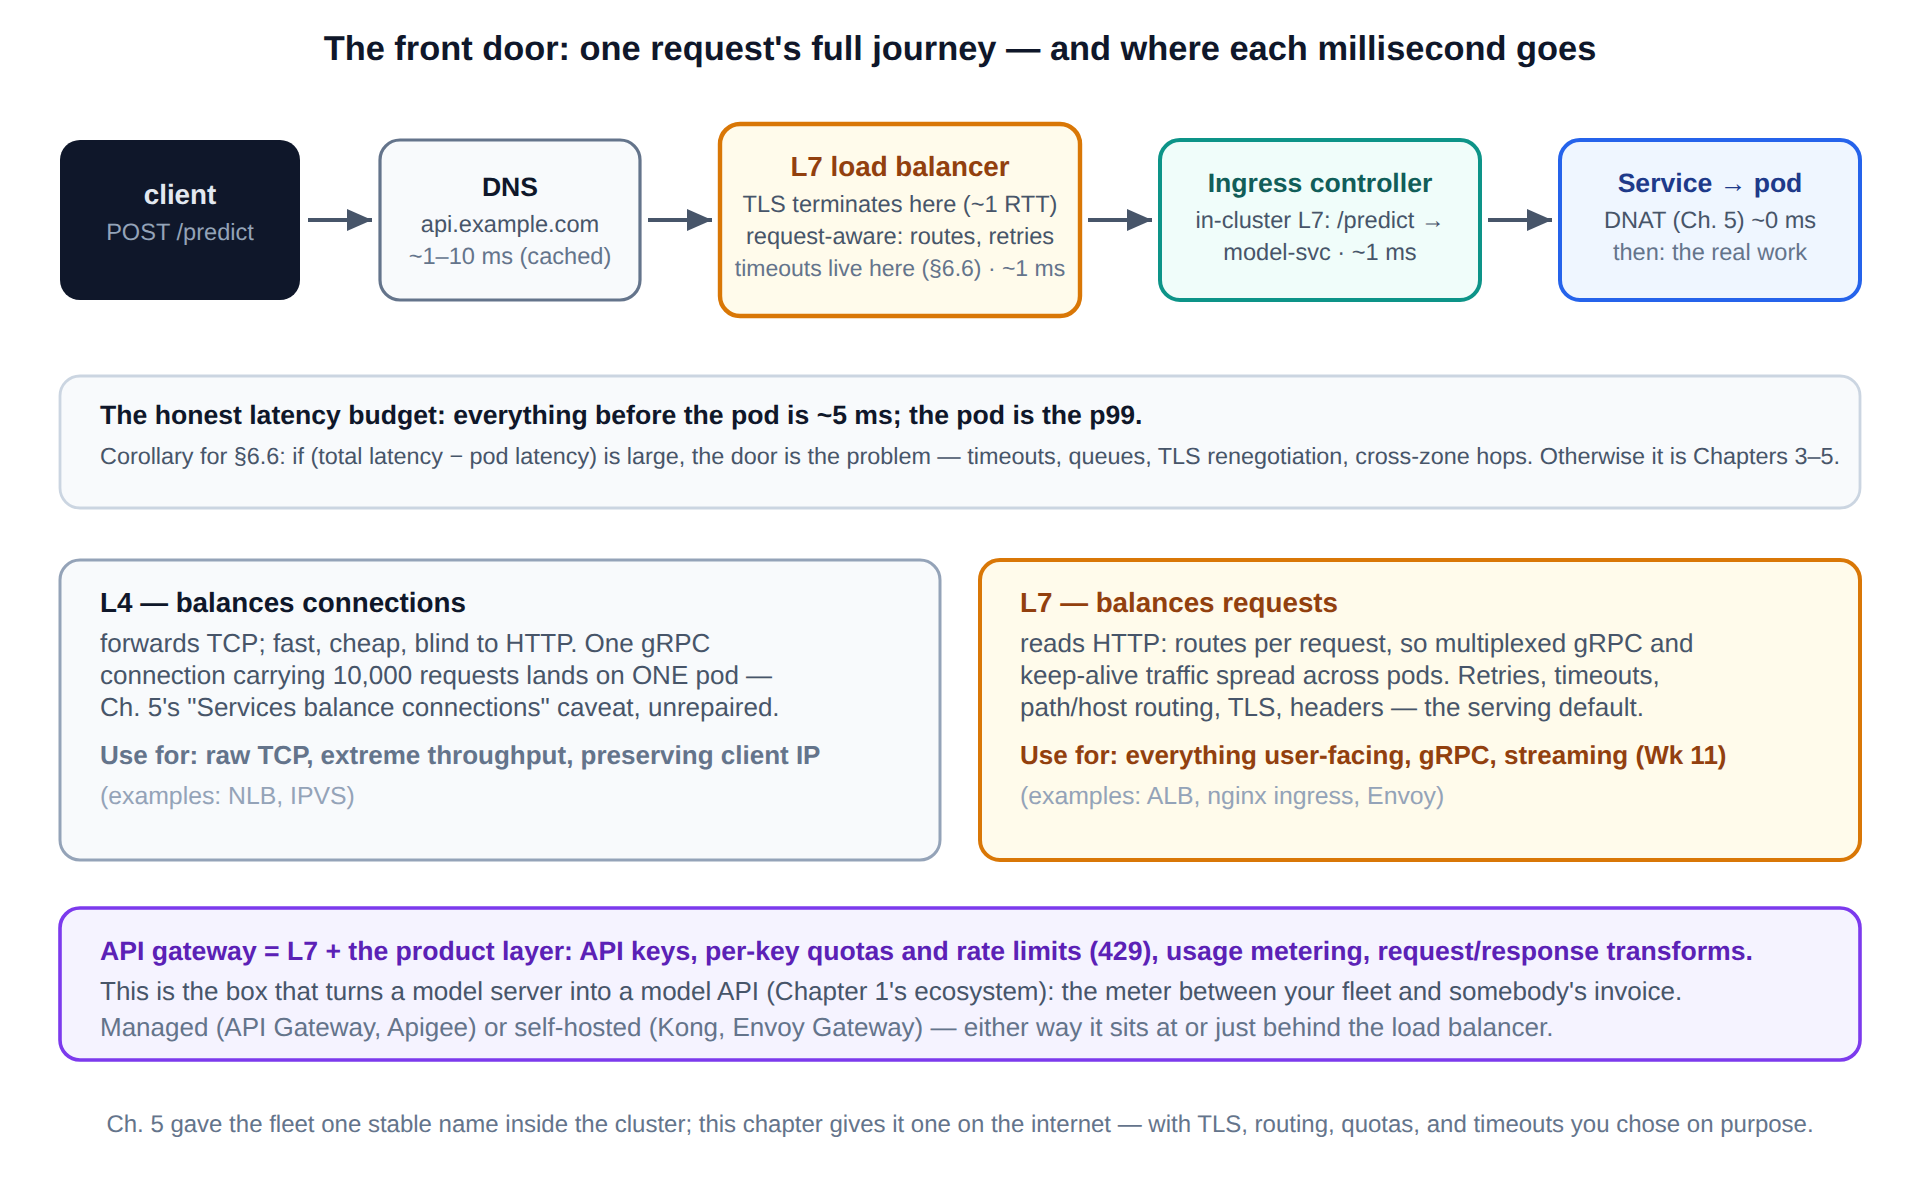
\includegraphics{figures/fig6-5_frontdoor.png}}\\[3pt]
  \figcaption{그림 6-5  요청의 여정. DNS → L7 로드 밸런서(TLS, 타임아웃) → Ingress(클러스터 내부 라우팅) → Service → 파드로 이어진다. 파드 전까지는 모두 합해 약 5 ms이고 p99는 파드에서 결정된다. §6.6에서는 이 사실을 진단 도구로 바꾼다.}
\end{tbbfigure}

\subsection*{L4 대 L7: 연결 대 요청}

로드 밸런서는 \textit{무엇을 읽는지}에 따라 두 종류로 나뉜다. \textbf{L4 로드 밸런서}는 전송 계층에서 동작한다. TCP 연결을 전달할 뿐 HTTP 바이트는 하나도 해석하지 않는다. 눈부시게 빠르고 저렴하며 프로토콜에 구애받지 않지만 지능은 딱 그 정도다. \textbf{L7 로드 밸런서}는 연결을 종료하고 \textit{요청을 읽어} 요청마다 새 결정을 내린다. 경로나 호스트로 라우팅하고, 멱등인 실패를 재시도하며, 헤더를 주입하고, TLS를 종료하고, 클라이언트와는 HTTP/2로, 파드와는 HTTP/1.1로 통신한다. 이 차이는 제5장이 주의사항을 남긴 바로 그 지점에서 빛을 발한다. Service(kube-proxy DNAT)는 \textbf{연결}을 로드 밸런싱한다. 따라서 다중화한 요청 만 개를 운반하는 장기 gRPC 채널 하나는 모두 단일 파드로 간다. 연결 유지 클라이언트 뒤의 플릿은 모든 대시보드가 "정상"이라고 말하는데도 부하가 극단적으로 불균형할 수 있다. L7 홉은 \textbf{요청} 수준에서 다시 로드 밸런싱해 정확히 이 문제를 고친다. 그래서 gRPC와 스트리밍 워크로드(11주 차)에는 L7 프록시가 부속품이 아니라 필수 요소다. 실용적으로는 필요할 때 원시 패킷 배관의 앞단에 L4를 두거나 클라우드에서 클러스터 내부 L7로 들어가는 입구로 쓰고, 요청이 중요한 단위인 곳에는 L7을 둔다. 서빙에서는 거의 모든 곳이 여기에 해당한다.

\subsection*{Ingress: 하나의 출입구, 여러 Service}

Service마다 클라우드 로드 밸런서를 하나씩 프로비저닝하는 것은 초보자가 튜토리얼에서 배우는 비싼 습관이다. 각 LB는 자체 IP와 유휴 비용이 있는 청구 대상 리소스다. Kubernetes의 답은 \textbf{Ingress}다. 여러 Service에 대응하는 호스트와 경로 규칙을 담은 라우팅 객체이며, \textbf{Ingress 컨트롤러}(nginx, Envoy 기반 컨트롤러, 또는 ALB를 직접 프로그래밍하는 클라우드 컨트롤러)가 실제로 구현한다. 로드 밸런서 하나가 클러스터에 들어오면 컨트롤러가 원하는 수의 Service로 요청을 분배한다. TLS 인증서는 호스트마다 붙이며 \code{cert-manager}가 발급과 갱신을 자동화한다. 실습에서 한 번 실행한 뒤에는 인증서를 다시 수동으로 관리하지 말자.

\begin{terminalbox}
\begin{Verbatim}[breaklines=true,breakanywhere=true,fontsize=\small,formatcom=\color{tbbtermfg},codes=\tbbcodeactive]
apiVersion: networking.k8s.io/v1
kind: Ingress
metadata:
  name: serving-ingress
  annotations:
    nginx.ingress.kubernetes.io/proxy-read-timeout: "120"
spec:
  tls:
  - hosts: [ api.example.com ]
    secretName: api-tls            # cert-manager fills this
  rules:
  - host: api.example.com
    http:
      paths:
      - path: /predict
        pathType: Prefix
        backend: { service: { name: model-svc, port: { number: 80 } } }
      - path: /embed
        pathType: Prefix
        backend: { service: { name: embed-svc, port: { number: 80 } } }

$ curl -sv https://api.example.com/predict -d '{"x":[1,2]}' 2>&1 \
    | grep -E "subject:|HTTP/"
*  subject: CN=api.example.com     # real TLS, terminated at the door
< HTTP/2 200
\end{Verbatim}
\end{terminalbox}
\figcaption{터미널 기록 6-8  Ingress 하나가 호스트의 TLS, 두 모델 Service로 가는 경로 라우팅, 의도적으로 설정한 타임아웃 어노테이션을 제공한다(기본값은 §6.6의 사고를 견디지 못한다). 이제 LB 하나가 네임스페이스 전체의 앞에 선다.}

\subsection*{API 게이트웨이: 제품이 사는 곳}

라우팅 위에는 \textbf{API 게이트웨이}가 있다. 기능상 L7 프록시이면서 \textit{제품}도 구현한다. API 키와 인증, 키별 속도 제한과 할당량(클라이언트가 존중하는 법을 배우게 될 \code{429 Too Many Requests}), 키·경로·토큰별 사용량 계측(청구서의 원재료), 요청 검증과 변환을 담당한다. 관리형 제품(AWS API Gateway, Apigee)과 자체 호스팅 제품(Kong, Envoy Gateway)은 운영 방식이 다를 뿐 개념은 같다. 이 책에서 게이트웨이는 제1장에서 시작한 고리를 닫는다. 계측되는 토큰, 계층별 할당량, 키를 제공하며 돈을 내고 사용하는 "모델 API 생태계"는 다른 조직의 플릿 앞에 놓인 \textit{바로 이 상자}다. 강의 프로젝트도 최소한 같은 형태를 요구한다. TLS 뒤에 키와 할당량을 갖춘 모델이 "curl에 응답하는 컨테이너"와 "누군가에게 비용을 청구할 수 있는 서비스"를 가른다. 중복에 관한 주의사항도 있다. 게이트웨이, Ingress, 메시(14주 차)는 모두 L7을 다루므로 성숙한 스택은 의도적으로 계층을 합친다. 경험 법칙은 약어마다 상자 하나를 두는 것이 아니라 \textit{관심사마다 소유자 하나}를 두는 것이다. TLS는 한 번만 종료하고, 속도 제한과 재시도는 각각 한곳에만 둔다.

\subsection*{타임아웃, 재시도, 연결 비우기: 추론을 망가뜨리는 설정}

출입구의 기본값은 수십 KB와 수백 ms인 웹페이지에 맞춰져 있으며 모델 서빙은 그 문장의 모든 가정을 어긴다. 대부분의 문제는 세 가지 설정에서 생긴다. \textbf{요청 타임아웃}: LB는 보통 30–60 s 안에 응답하지 않은 상위 서버를 포기하고 \code{504}를 반환한다. 제3장에서 추론 지연 시간에는 배치와 길이에 비례해 치솟는 \textit{형태}가 있다고 배웠다. 따라서 타임아웃은 최악 입력에서 측정한 정직한 p99(제1장의 SLO 규율)보다 길어야 한다. 그렇지 않으면 긴 요청은 출입구에서 죽고 GPU는 아무도 받지 않을 작업을 마친다. \textbf{유휴 타임아웃(idle timeout)}: 대부분의 LB는 N초 동안 \textit{바이트가 하나도 움직이지 않는} 연결을 별도로 정리한다(ALB 기본값: 60초). 생성 도중 토큰 사이에서 70 s 멈추는 스트리밍 LLM 응답(11주 차)은 이 제한에 걸린다. §6.6의 징후대로 연결이 \textit{정확히} N초에 끊긴다. 유휴 타임아웃을 늘리거나 연결 유지 프레임을 보내 해결한다. \textbf{재시도}: L7 출입구는 눈에 띄지 않게 실패를 재시도할 수 있다. 멱등 GET에는 선물이지만 추론에는 위험하다. 30초짜리 생성을 재시도하면 시스템이 느려진 바로 그때 GPU 부하가 \textit{두 배}가 된다. 게이트웨이 × 클라이언트 두 계층에서 타임아웃을 각각 재시도하면 3 × 3 = 사용자 동작 하나당 아홉 번 시도가 된다. 필요한 규율은 \textbf{재시도 예산(retry budget)}이다. 타임아웃은 절대 재시도하지 않고 연결 수준의 실패만 단일 계층에서 지터(jitter)를 넣은 지수 백오프(exponential backoff)와 함께 재시도한다. 9주 차 부하 테스트에서는 재시도 폭풍(retry storm)을 의도적으로 만들어 파형을 익힌다.

네 번째 설정은 모든 팀이 언젠가 만나는 증상인 \textbf{롤아웃 중 정확히 발생하는 502 급증}을 설명하므로 문단 하나를 온전히 쓸 가치가 있다. 연결을 비우는 두 시계가 일치해야 한다. LB는 자체 지연(\code{deregistration delay} / connection draining) 뒤 종료 중인 파드를 등록 해제하고, Kubernetes는 \code{terminationGracePeriodSeconds} 뒤 파드를 죽인다(제5장의 과정). LB가 여전히 유효한 대상으로 보는 동안 파드가 죽으면, 즉 유예 시간이 너무 짧거나 지연이 너무 길거나 서버가 SIGTERM을 보자마자 연결을 비우지 않고 종료하면(제3장의 핸들러가 다시 등장한다), 처리 중 요청이 시체에 부딪히고 출입구가 502를 보고한다. 해결책은 시계를 맞추는 것이다. 먼저 준비 상태 검사가 실패해 엔드포인트에서 빠지고 트래픽 유입이 멈춘다. 그런 다음 처리 중 작업을 비운 뒤 종료한다. 유예 기간은 가장 긴 정당한 요청보다 길어야 한다. 이 문장의 모든 계층은 이미 읽은 장에 있으며, 출입구는 불일치를 고객에게 보이게 할 뿐이다.

\begin{terminalbox}
\begin{Verbatim}[breaklines=true,breakanywhere=true,fontsize=\small,formatcom=\color{tbbtermfg},codes=\tbbcodeactive]
# the streaming incident, reproduced on purpose (lab, part C):
$ time curl -sN https://api.example.com/generate -d '{"n_tokens": 999}'
...tokens......tokens.......                       # then silence...
curl: (18) transfer closed with outstanding read data remaining
real  1m0.02s                       # <- suspiciously exactly 60s
# repeat it: 60.01s. 60.02s. the roundness IS the diagnosis:
# no bytes moved for idle-timeout seconds -> the LB reaped it.
$ kubectl annotate ingress serving-ingress \
    nginx.ingress.kubernetes.io/proxy-read-timeout="300" --overwrite
$ time curl -sN https://api.example.com/generate -d '{"n_tokens": 999}'
real  1m34.8s                       # the stream now outlives its pauses
\end{Verbatim}
\end{terminalbox}
\figcaption{터미널 기록 6-9  유휴 타임아웃에 의한 끊김. 정확히 60.0 s에 두 번 죽는 스트림은 서버 버그가 아니라 출입구의 기본값 때문이다. 11주 차 토큰 스트림의 생사는 이 설정에 달렸다.}

\begin{calloutbox}{tbbpurple}{tbbpurplefill}
{\normalsize\bfseries\color{tbbpurple}생각해 보기}\par\vspace{3pt}
\begin{tbbitemize}
  \item 상태 확인도 요청이다. LB 노드 2개 × 10초마다 × 대상 20개에 kubelet의 준비 상태 프로브까지 더해 백그라운드 QPS를 계산하자. 그런 다음 상태 확인을 실제 부하로 바꾸는 실수를 말하자. 순전파를 실행하는 비싼 /healthz를 생각하면 된다.
  \item p99가 8 s지만 가장 큰 배치와 길이를 사용한 최악의 정당한 요청은 45 s가 걸리는 서비스의 타임아웃 사다리를 설계하자. 클라이언트, 게이트웨이, LB 요청, uvicorn 타임아웃 가운데 무엇이 가장 커야 하며, 순서가 선택 사항이 아닌 이유는 무엇인가?
  \item 게이트웨이는 연결 실패를 한 번 재시도하고 클라이언트 라이브러리는 모든 5xx를 두 번 재시도하며 메시(14주 차)도 자체 재시도를 추가한다. 피크 부하에서 노드가 죽었다. 요청이 어떻게 늘어나고 플릿이 실제로 어떤 부하를 보는지 그린 뒤, 강제할 한 문장짜리 재시도 정책을 작성하자.
\end{tbbitemize}
\end{calloutbox}

\section{경계: VPC, 보안 그룹, 저렴한 경로}

지금까지는 패킷이 흐를 수 있다고 가정했다. 이 절에서는 \textit{어떤} 패킷이 흐를 수 있는지 정한다. 결정 단위는 클라우드 네트워크의 사설 영역인 \textbf{VPC}다. \code{10.0.0.0/\allowbreak 16} 같은 주소 공간을 고르고 가용 영역별 \textbf{서브넷(subnet)}으로 나눈 뒤 \textbf{라우팅 테이블}로 연결한다. 라우팅 테이블 항목 두 개가 두 가지 서브넷을 정의한다. \textbf{공개 서브넷}은 \code{0.0.0.0/\allowbreak 0}을 \textit{인터넷 게이트웨이}로 라우팅하므로 내부의 리소스가 공개 IP를 갖고 외부에서 접근될 수 있다. \textbf{사설 서브넷}에는 그런 경로가 없다. 인스턴스에 공개 IP가 없고, 방화벽 관리자의 성실함이 아니라 \textit{구조 자체로} 인터넷에서 접근할 수 없다. 서빙에 적합한 자세도 곧바로 나온다. 그림 6-6처럼 \textbf{로드 밸런서만 공개하고 GPU 플릿은 사설 영역에 둔다.} 시간당 \$30인 공개 IP 노드는 결제 계정이 붙은 공격 표면이지만 사설 노드는 공격자가 접근할 수 없다.

\begin{tbbfigure}
  \adjustbox{max width=0.94\linewidth,max totalheight=0.46\textheight}{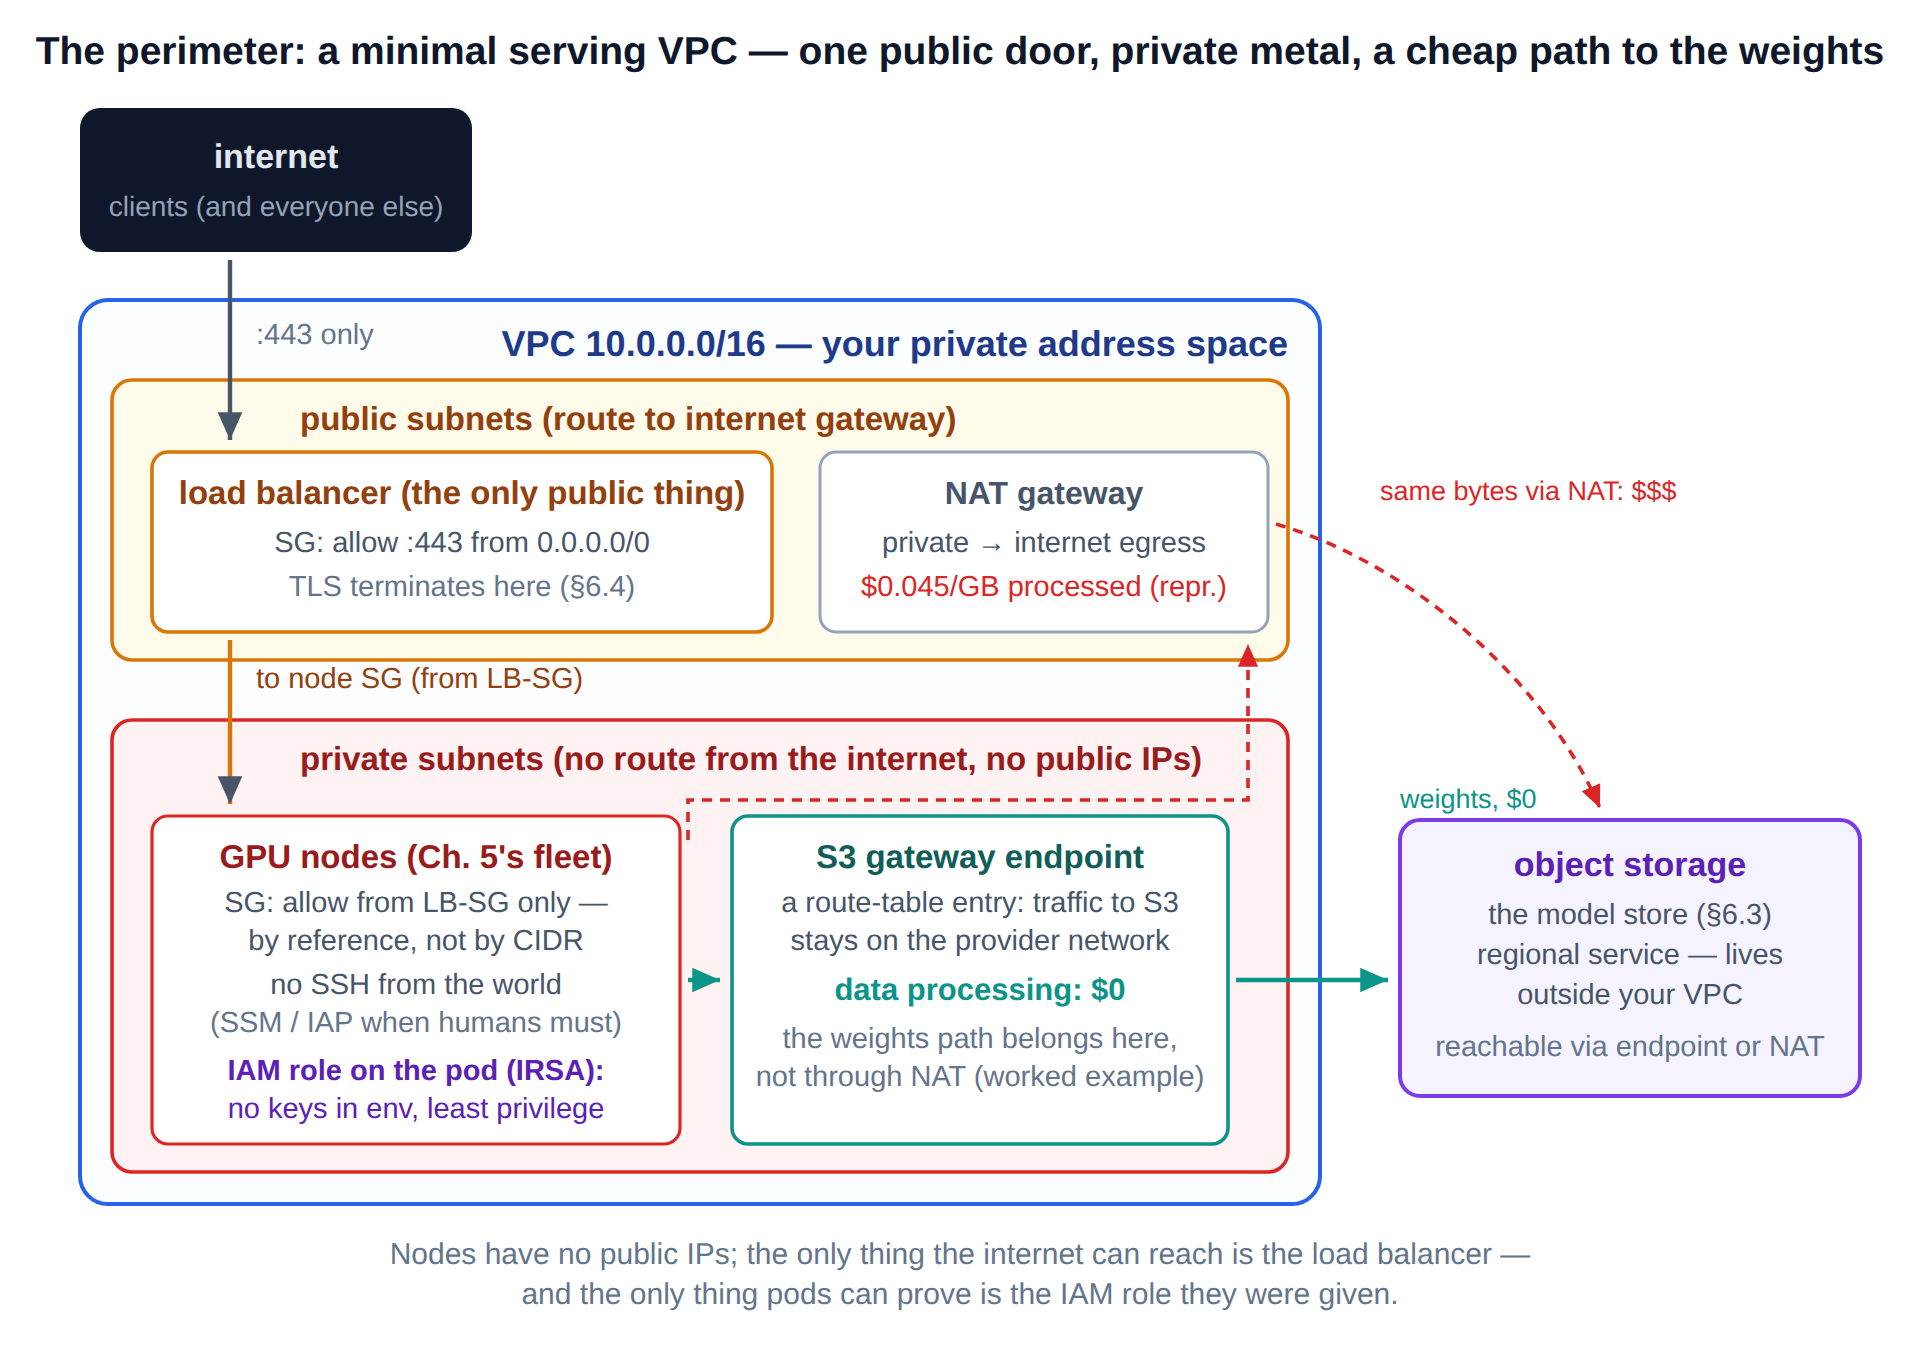
\includegraphics{figures/fig6-6_vpc.png}}\\[3pt]
  \figcaption{그림 6-6  최소 서빙 VPC. 공개 출입구 하나(LB), 사설 하드웨어(플릿), 모델 스토어로 가는 두 경로인 무료 게이트웨이 엔드포인트와 사용량에 따라 과금되는 NAT 우회로로 구성된다. 의도적으로 선택해야 한다.}
\end{tbbfigure}

\subsection*{보안 그룹: 참조로 연결하는 상태 저장 허용 목록}

VPC 안에서 \textbf{보안 그룹}(SG)은 인스턴스별 방화벽이며, 세 가지 성질이 핵심이다. 첫째, \textbf{허용 전용}이다. SG는 연결을 허용할 포트, 프로토콜, 출발지를 나열하고 목록에 없는 것은 모두 거부하므로 "거부 규칙 순서" 퍼즐이 없다. 둘째, \textbf{상태를 저장}한다. 인바운드 연결을 허용하면 응답 패킷은 자동으로 흐른다. 클라우드는 제3장의 \code{-p 8080:8000} 경로에서 본 conntrack과 똑같이, 추상화 한 단계 위에서 연결을 추적한다. 셋째, 아키텍처를 읽기 쉽게 하는 성질로 \textbf{출발지에는 CIDR 범위뿐 아니라 다른 SG도 지정할 수 있다.} 서빙 연결 고리는 세 문장으로 정리된다. LB의 SG는 \code{0.0.0.0/\allowbreak 0}에서 오는 \code{:443}을 허용한다. 노드의 SG는 \textit{LB의 SG에서} 오는 서비스 포트를 허용한다. LB가 확장되거나 이동할 때 조용히 바뀌는 IP 범위가 아니라 SG를 참조한다. SSH는 어디에서 오든 허용하지 않으며, 사람이 꼭 들어가야 할 때는 감사 기록이 남는 SSM/IAP 세션 도구를 사용한다. 참조 연결은 인프라가 바뀌어도 의도를 보존한다. 내일 로드 밸런서의 IP가 무엇이든 "노드는 \textit{로드 밸런서에서} 오는 트래픽을 허용한다"는 사실이 유지된다. (SG 아래에는 상태가 없고 서브넷 수준에서 규칙 번호로 동작하는 네트워크 ACL도 있다. 관례상 열어 두고 SG로 의도를 표현하며, 서브넷 전체를 거칠게 차단할 때만 NACL을 사용한다.)

\begin{terminalbox}
\begin{Verbatim}[breaklines=true,breakanywhere=true,fontsize=\small,formatcom=\color{tbbtermfg},codes=\tbbcodeactive]
# perimeter, demonstrated: (1) the node, from the internet:
$ curl -m 5 http://203.0.113.40:30080/predict
curl: (28) Connection timed out       # no route, no public IP. good.
# (2) the door, from the internet:
$ curl -s https://api.example.com/predict -d '{"x":[1,2]}'
{"y": 0.87, "model": "v8"}            # the one sanctioned path
# (3) identity, from inside a pod - no keys anywhere:
$ kubectl exec -it model-server-...-2xk4p -- \
    aws sts get-caller-identity --query Arn --output text
arn:aws:sts::1234:assumed-role/model-server-irsa/...
$ kubectl exec -it model-server-...-2xk4p -- \
    aws s3 ls s3://ml-models/bert-classifier/v8/   # allowed prefix
2026-07-02  461301120 model.safetensors
$ kubectl exec -it model-server-...-2xk4p -- \
    aws s3 ls s3://corp-finance-exports/
An error occurred (AccessDenied)      # least privilege, working
\end{Verbatim}
\end{terminalbox}
\figcaption{터미널 기록 6-10  세 가지 프로브로 살펴본 경계. 외부에서 접근할 수 없는 노드, 응답하는 LB, 범위가 제한된 IAM 역할만 자격 증명으로 가진 파드가 보인다. 애초에 비밀 값이 아니었으므로 외부로 빼돌릴 수도 없다.}

\subsection*{키 없는 아이덴티티와 가중치가 지나야 할 경로}

터미널 기록의 세 번째 프로브는 자세히 풀어 볼 가치가 있다. 서빙 시스템이 팀을 가장 자주 곤란하게 하는 부분이 자격 증명 처리이기 때문이다. 안티패턴은 환경 변수에 액세스 키를 넣는 것이다. 수명이 길고 복사해서 붙여 넣을 수 있으며 모든 \code{kubectl describe}와 충돌 덤프에 노출되지만 한 번도 교체하지 않는다. 권장 패턴은 \textbf{워크로드 아이덴티티}(EKS의 IRSA, GKE의 Workload Identity)다. 제5장의 객체 목록에 나온 Kubernetes 아이덴티티인 파드의 \textit{서비스 계정}을 IAM 역할에 바인딩하면, 파드 안의 클라우드 SDK가 토큰 체인을 통해 수명이 짧은 자격 증명을 자동으로 얻는다. 누출할 것도 교체할 것도 없다. 운영상 특히 중요한 점은 \textbf{최소 권한을 워크로드별로 적용}할 수 있다는 것이다. 모델 서버 역할은 \code{ml-models/\allowbreak bert-classifier/\allowbreak *}만 읽고, 로더는 읽을 수 있지만 쓸 수 없으며, 다른 곳의 학습 파이프라인은 새 접두사를 쓸 수 있지만 덮어쓸 수 없다. §6.3의 변경 불가능성 규율을 팀 규범에서 강제 속성으로 바꾼다.

마지막으로 비용을 살펴보자. 사설 서브넷에서 인터넷으로 나가는 트래픽은 \textbf{NAT 게이트웨이(NAT gateway)}를 통과하고, NAT 게이트웨이는 시간당 비용에 더해 \textbf{처리한 GB마다} 비용을 받는다(대표값 GB당 약 \$0.045). 함정은 S3가 VPC \textit{밖에} 있다는 점이다. 그래서 사설 노드가 S3에서 13 GB 가중치를 가져오는 트래픽은 \textit{기본적으로} NAT 경로를 탄다. 해결책은 \textbf{게이트웨이 VPC 엔드포인트}다. S3/DynamoDB로 가는 트래픽을 제공자 백본을 통해 직접 보내는 라우팅 테이블 항목으로, \textbf{데이터 처리 비용이 0}이고 보통 처리량도 더 높다. ML 인프라에서 투자 대비 수익이 가장 큰 네트워크 설정 한 줄이라고 해도 과언이 아니다.

\begin{calloutbox}{tbbred}{tbbamberfill}
{\normalsize\bfseries\color{tbbamberdark}계산 예시 — 가중치에 붙는 NAT 세금}\par\vspace{3pt}
노드 20개 플릿이 매일 배포할 때마다 13 GB 모델을 다시 가져오고 오토스케일링에 따른 교체도 생긴다. 하루에 노드 가져오기 25회라 하면 S3 → 노드 트래픽은 \textbf{하루 325 GB}다.

\begin{tbbitemize}
  \item \textbf{NAT 게이트웨이 경유:} 325 GB × \$0.045 ≈ 하루 \$14.6 ≈ \textbf{월 \$440}다. 제공자 네트워크를 떠나지도 않은 바이트에 내는 비용이다. NAT 자체의 시간당 약 \$0.045, 즉 월 약 \$32의 기본료도 더해진다.
  \item \textbf{S3 게이트웨이 엔드포인트 경유:} 생성 시 라우팅 테이블 항목 하나만 추가하면 같은 바이트가 \textbf{\$0.00}이다.
\end{tbbitemize}

같은 아키텍처와 같은 트래픽에서 연간 약 \$5,000 차이가 난다. 더구나 실패는 조용하다. NAT를 통해서도 모든 것이 \textit{동작}하지만 비용이 청구될 뿐이다. 점검 규칙은 S3와 통신하는 사설 서브넷에 첫날부터 게이트웨이 엔드포인트를 두는 것이다. (리전 간 전송은 별도의 세금이다. 모델 스토어를 플릿과 같은 리전에 두지 않으면 GB당 약 \$0.02와 추가 지연 시간을 내야 한다. 12주 차 다중 리전 주제에서 다룬다.)
\end{calloutbox}

\vspace{3.0pt}

\begin{calloutbox}{tbbpurple}{tbbpurplefill}
{\normalsize\bfseries\color{tbbpurple}생각해 보기}\par\vspace{3pt}
\begin{tbbitemize}
  \item "노드 SG는 LB SG의 트래픽을 허용한다"가 "LB 서브넷의 CIDR에서 오는 트래픽을 허용한다"보다 확실히 나은 이유는 무엇인가? 시간이 지나면서 CIDR 규칙에 생기는 실패와 SG 참조에는 그 실패가 생길 수 없는 이유를 말하자.
  \item 공격자가 서빙 파드 안에서 코드 실행에 성공했다(악성 pickle로 7주 차 형식 경고가 현실이 됨). (a) 환경 변수에 s3:* 권한이 있는 액세스 키를 둔 경우와 (b) 접두사 하나의 읽기 전용으로 범위를 제한한 IRSA의 장애 영향 범위를 비교하자. 각각 어디까지 접근할 수 있으며 제3장의 공유 커널 주의사항은 무엇을 더하는가?
  \item 청구서에서 NAT 게이트웨이가 GPU 다음이자 스토리지보다 큰 세 번째 항목이다. 가능한 트래픽(가중치, 이미지 가져오기, 빌드 때의 pip 설치, 원격 측정)을 재구성하고, 그 가운데 게이트웨이 엔드포인트가 해결하는 것과 레지스트리 미러 또는 인터페이스 엔드포인트가 필요한 것을 구분하자.
\end{tbbitemize}
\end{calloutbox}

\section{출입구 읽기: 상태 코드 현장 안내서}

제5장의 현장 안내서는 클러스터 안에서 파드 상태를 읽는 법을 가르쳤다. 이 장의 실패는 \textit{바깥}에서 자신을 알린다. 사용자, 합성 검사, 또는 14주 차 경보가 상태 코드 하나만 건네준다. 제5장과 마찬가지로 좋은 소식이 있다. §6.4 출입구의 각 계층은 자기 어휘로만 실패하므로 명령을 하나도 실행하기 전에 \textbf{코드가 실패 위치를 좁혀 준다.} 포렌식을 시작하기 전 검색 공간을 절반으로 줄이는 동작도 하나 있다. \textbf{내부에서 요청을 다시 실행}한다(\code{kubectl port-forward}로 파드에 직접 연결). 내부는 정상이고 외부만 고장이라면 TLS, 라우팅, 타임아웃, 상태 확인, 경계 같은 출입구 문제다. 둘 다 고장이면 플릿 문제이며, 단서를 하나 얻은 채 제5장의 안내서로 돌아간다(그림 6-7).

\begin{tbbfigure}
  \adjustbox{max width=0.94\linewidth,max totalheight=0.46\textheight}{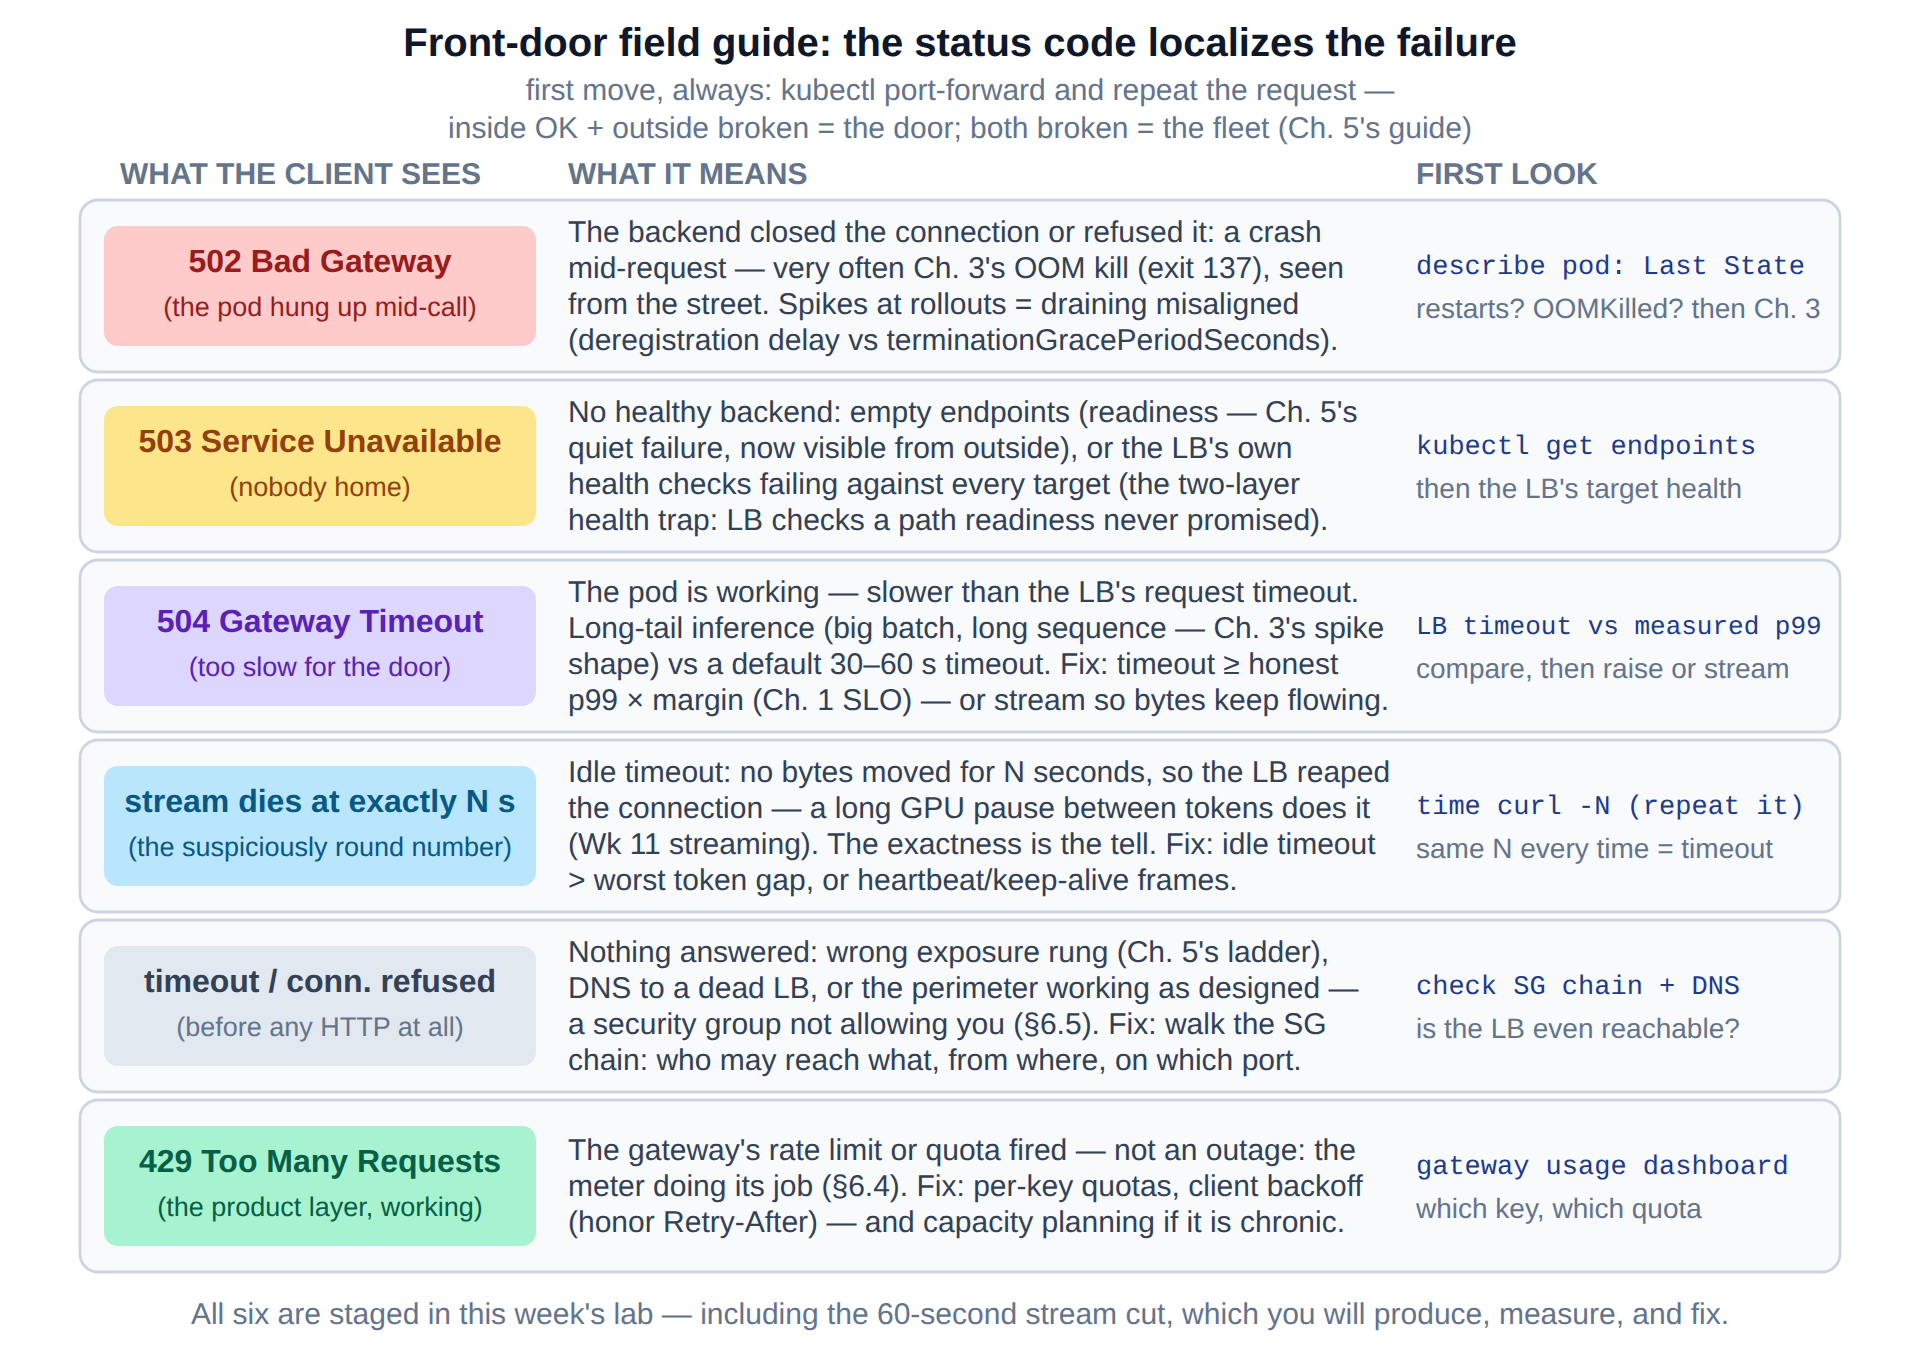
\includegraphics{figures/fig6-7_fieldguide.png}}\\[3pt]
  \figcaption{그림 6-7  해독표. 502(파드가 연결을 끊음), 503(응답할 대상 없음), 504(출입구 기준으로 너무 느림), 정확히 N초에 끊기는 스트림, 조용한 연결 타임아웃, 429(정상 작동하는 계량기)를 정리했다. 실습에서 모두 재현한다.}
\end{tbbfigure}

\subsection*{포렌식 따라 하기: 대시보드는 초록색인데 503}

\begin{terminalbox}
\begin{Verbatim}[breaklines=true,breakanywhere=true,fontsize=\small,formatcom=\color{tbbtermfg},codes=\tbbcodeactive]
$ curl -s -o /dev/null -w "%{http_code}\n" \
    https://api.example.com/predict -d '{"x":[1,2]}'
503                                  # "Service Unavailable" - from whom?
$ kubectl get pods -l app=model      # the fleet looks... fine?
NAME                            READY   STATUS    RESTARTS   AGE
model-server-59d8c7f9b6-2xk4p   1/1     Running   0          3h
model-server-59d8c7f9b6-m7qvw   1/1     Running   0          3h
$ kubectl port-forward pod/model-server-59d8c7f9b6-2xk4p 8000:8000 &
$ curl -s -o /dev/null -w "%{http_code}\n" \
    localhost:8000/predict -d '{"x":[1,2]}'
200                                  # inside OK + outside broken = DOOR
$ kubectl describe ingress serving-ingress | grep -A2 Backends
  /predict   model-svc:80   (<none>)          # <- the controller sees
$ kubectl get endpoints model-svc               #    no endpoints...
NAME        ENDPOINTS   AGE
model-svc   <none>      3h                      # Ch. 5's quiet failure -
# a readiness typo after this morning's change - now visible as a 503
# to every customer. fix the probe path; endpoints repopulate; 200.
\end{Verbatim}
\end{terminalbox}
\figcaption{터미널 기록 6-11  검색 공간을 나누는 동작. 외부는 503이고 포트 포워딩은 200이므로 출입구 문제다. 이어서 출입구 자체의 증거인 Ingress 백엔드 목록과 비어 있는 엔드포인트를 확인한다. 제5장의 조용한 실패를 거리에서 바라본 모습이다.}

터미널 기록처럼 연결 고리를 따라가면 각 홉이 질문 하나에 답한다. \textbf{상태 코드}는 실패 계층의 어휘를 알려 준다. \code{503}은 프록시가 "정상 상위 서버가 없다"고 말하는 것으로, DNS나 TLS가 아니라 엔드포인트, 준비 상태, 또는 LB 자체 상태 확인을 가리킨다. \textbf{포트 포워딩 프로브}는 파드가 서빙할 수 있음을 증명해 "API가 중단되었다"를 "출입구에 보낼 대상이 없다"로 바꾼다. 마지막으로 제5장에서 가장 가치 있는 습관인 \textbf{엔드포인트 확인}이 원인을 찾는다. 두 장이 하나의 진단 언어로 이어진다. 이 책의 인프라 절반을 \textit{완성}한다는 의미가 바로 이것이다.

\subsection*{제3–5장에 뿌리를 둔 나머지 해독표}

\begin{tbbitemize}
  \item \textbf{502 Bad Gateway — 호출 도중 파드가 연결을 끊었다.} 출입구는 연결했지만 백엔드가 닫거나 거부했다. 이미 아는 원인은 요청 중 충돌, 흔히 제3장의 OOM 강제 종료(종료 코드 137: 먼저 \code{Last State} 확인), 또는 §6.4의 롤아웃 시계 불일치다. LB가 여전히 대상으로 보는 동안 파드가 죽었다면 등록 해제 지연과 \code{terminationGracePeriodSeconds}를 비교하고 서버가 SIGTERM 뒤 연결을 비우는지 확인한다. \textit{배포 시점에 급증하는 502는 반증될 때까지 연결 비우기(connection draining) 버그다.}
  \item \textbf{504 Gateway Timeout — 출입구가 보기에는 너무 느리다.} 파드는 작업 중이지만 출입구가 먼저 포기했다. 제3장은 추론 지연 시간의 급증 형태(배치 × 시퀀스)를 보여 주었고 제1장은 SLO 언어를 제공했다. 해결책은 "LB/Ingress 요청 타임아웃을 정직하게 측정한 최악 p99보다 높이거나, 입력에 상한을 두거나, 바이트가 계속 흐르도록 스트리밍한다"다. 시스템이 가장 느릴 때 GPU 부하를 두 배로 만드는 "재시도 추가"는 답이 아니다(§6.4의 예산).
  \item \textbf{정확히 N초에 죽는 스트림} — §6.4의 유휴 타임아웃이며 딱 떨어지는 시간 자체가 진단의 전부다. 두 번 재현하고 숫자를 읽은 뒤 유휴 타임아웃을 늘리거나 연결 유지 프레임을 추가한다. 11주 차 토큰 스트림 때문에 이 책에서 가장 많이 재현하는 터미널 기록이 된다.
  \item \textbf{연결 타임아웃 / 거부 — HTTP에 도달하기 전.} 아무것도 응답하지 않았다. 잘못된 노출 단계(제5장의 사다리), 삭제된 LB를 가리키는 DNS, 또는 예상과 달리 자신을 상대로 \textit{설계대로 동작하는} §6.5의 경계가 원인이다. 사무실 IP 범위를 한 번도 허용하지 않은 SG나 공개라고 생각한 사설 엔드포인트가 예다. 누가 어디에서 어떤 포트로 무엇에 접근할 수 있는지 SG 연결 고리를 따라간다.
  \item \textbf{429 Too Many Requests — 제품 계층이 정상 작동한다.} 게이트웨이의 키별 할당량이 발동했다. 장애가 아니라 플릿과 청구서를 보호하는 계량기다. 클라이언트는 \code{Retry-After}를 지키고 지터를 넣은 백오프를 추가한다. 운영자는 현실에 맞는 키별 할당량을 설정하고 정상 사용량에서도 429가 계속되면 용량을 계획한다.
\end{tbbitemize}

\subsection*{두 계층 상태 확인의 함정}

한 가지 실패는 내부에서 보이지 않으므로 별도의 하위 절로 다룰 가치가 있다. 클라우드 LB는 Kubernetes 준비 상태와 독립적으로 대상에 \textbf{자체 상태 확인}을 실행한다. 두 상태 판단이 어긋날 수 있다. LB가 서버에 없는 \code{/\allowbreak health}를 검사해 404를 "비정상"으로 해석하거나, kube-proxy가 다른 곳으로 라우팅하는 노드의 NodePort를 검사하거나, 준비 상태보다 더 엄격한 타임아웃을 사용할 수 있다. 그 결과 \textbf{kubectl은 모두 준비 상태라고 표시하지만 LB의 정상 대상은 0이고 고객은 503을 본다.} 터미널 기록 6-11과 증상은 같지만 원인이 다르다. \code{kubectl get endpoints}에는 대상이 \textit{채워져} 나오므로 특히 혼란스럽다. 예방 규칙은 \textbf{상태 확인 엔드포인트 하나를 유일한 진실의 원천으로 삼는 것}이다. LB의 검사 경로, 준비 상태 프로브, 게이트웨이 검사가 모두 같은 의미의 \code{/\allowbreak ready}를 가리키게 한다. 실습에서 이 상황을 재현할 때 증거의 위치를 주목하자. Kubernetes 안이 아니라 LB의 대상 상태 콘솔에 있다. 이 책에서 처음으로 클러스터 밖의 제어판으로 이동하는 순간이며, 거부할 수 있는 모든 계층을 관측 가능성이 포괄해야 한다는 14주 차 주제를 미리 보여 준다.

\begin{tbbtablewrap}
  \begin{tabular}{@{}>{\raggedright\arraybackslash}m{\dimexpr 0.2181\tbltextwidth-2\tabcolsep\relax} >{\raggedright\arraybackslash}m{\dimexpr 0.3670\tbltextwidth-2\tabcolsep\relax} >{\raggedright\arraybackslash}m{\dimexpr 0.4149\tbltextwidth-2\tabcolsep\relax}@{}}
  \arrayrulecolor{tbbnavy}\specialrule{1pt}{0pt}{0pt}
  \rowcolor{tbbtablehead}{\centering \bfseries\color{tbbnavy}신호} & {\centering \bfseries\color{tbbnavy}출입구의 의미} & {\centering \bfseries\color{tbbnavy}우선 확인 항목} \\
  \arrayrulecolor{tbbnavy}\specialrule{0.7pt}{0pt}{2pt}
  {\textbf{502}} & {백엔드가 호출 도중 닫거나 거부} & {파드 재시작, Last State(OOM 137?), 롤아웃 연결 비우기 시계} \\
  \arrayrulecolor{tbbtableborder}\hline
  {\textbf{503}} & {정상 상위 서버가 전혀 없음} & {kubectl get endpoints, 이어서 LB 대상 상태(두 계층 함정)} \\
  \arrayrulecolor{tbbtableborder}\hline
  {\textbf{504}} & {상위 서버가 출입구 타임아웃보다 느림} & {LB/Ingress 타임아웃과 측정한 최악 p99 비교} \\
  \arrayrulecolor{tbbtableborder}\hline
  {\textbf{정확히 N s에 끊김}} & {N s 동안 바이트 없음 → 유휴 정리} & {time curl -N을 두 번, 유휴 타임아웃 상향 / 연결 유지} \\
  \arrayrulecolor{tbbtableborder}\hline
  {\textbf{타임아웃, HTTP 없음}} & {출입구에 도달하지 못함} & {DNS → SG 연결 고리 → 노출 단계(제5장 사다리)} \\
  \arrayrulecolor{tbbtableborder}\hline
  {\textbf{429}} & {설계대로 할당량 강제} & {키별 게이트웨이 사용량, Retry-After에 따른 클라이언트 백오프} \\
  \arrayrulecolor{tbbnavy}\specialrule{1pt}{2pt}{0pt}
  \end{tabular}\par
  \figcaption{표 6-3  한눈에 보는 출입구 오류 어휘}
\end{tbbtablewrap}

\begin{calloutbox}{tbbpurple}{tbbpurplefill}
{\normalsize\bfseries\color{tbbpurple}생각해 보기}\par\vspace{3pt}
\begin{tbbitemize}
  \item 사용자가 배포와 무관하게 요청의 약 1\%에서 간헐적인 502가 발생한다고 보고했다. 파드 재시작은 0이다. 이 절을 바탕으로 의심 목록을 만들고 구별할 측정값을 제시하자. 어떤 파드가 긴 요청을 처리하는지, LB 연결 재사용, uvicorn 워커 재활용을 생각해 보자.
  \item 합성 검사(14주 차)는 고객보다 \textit{먼저} 표 6-3의 각 행을 찾아야 한다. 503, 504, 스트림 끊김을 함께 포괄하는 프로브 세 개의 경로, 주기, 경보 조건을 설계하고, 각 프로브가 유효하려면 어느 계층 밖에서 실행되어야 하는지 밝히자.
  \item 두 계층 상태 확인 함정은 증거를 Kubernetes 밖에 두었다. 그림 6-5에서 kubectl 사용자가 볼 수 없는 상태를 유지하는 모든 계층을 나열하고, 각 계층에서 "여기는 초록색인데 저기는 빨간색"이 무엇을 뜻하는지 설명하자.
\end{tbbitemize}
\end{calloutbox}

\section{실습: S3에서 로딩하는 서빙 구조 완성}

이번 주 강의계획서의 문구는 "S3에서 모델을 로딩하는 서빙 구조를 완성한다"이며, 핵심 단어는 \textit{완성}이다. 실습을 마치면 스토어 → 로더 → 플릿 → Service → 출입구로 이어지는 이 책의 서빙 골격이 노트북에서 처음부터 끝까지 존재하고, 모든 연결부에 실제 측정값이 생긴다. 스토리지 절반은 minikube 클러스터 안에 배포한 S3 호환 저장소 \textbf{MinIO}를 사용한다. 같은 API와 SDK를 쓰고 \code{aws} 대신 \code{mc}를 사용하며 비용은 0이다. 클라우드 경계 절반은 §6.5의 체크리스트로 진행하고, 크레딧이 있는 팀을 위해 관리형 클러스터 선택 부록을 제공한다. 전체 과정은 \code{ml} 네임스페이스에서 작업한다.

\subsection*{파트 A — 스토어를 세우고 로더를 정직하게 만들기}

강의 매니페스트로 MinIO를 배포한다. Deployment, Service, PVC로 구성되어 있으며 모든 객체가 제5장의 명사이므로 읽어 보자. 버킷을 만들고 실습 모델을 \textbf{두 번}, 즉 매니페스트가 있는 \code{v7/\allowbreak }과 \code{v8/\allowbreak } 접두사로 업로드한다. \code{mc mb}, \code{mc cp}, \code{mc ls}를 사용해 첫 순간부터 변경 불가능성 규율을 연습한다. 이어서 이번 주의 기준이 될 측정을 수행한다. 제공된 순진한 로더(스트림 하나)를 4 GB 실습 모델에 실행해 시간을 기록한다. 이를 N개의 동시 범위 GET으로 확장한다. 유인물은 스레드 풀 골격을 제공하고 범위 계산과 재조립은 직접 작성한다. N ∈ \{1, 4, 8, 16, 32\}를 훑어 시간 대 N 그래프를 그리고 굴곡점을 찾는다. 마지막으로 승리를 선언하기 전에 \code{manifest.json} 체크섬으로 모든 파일을 검증한다. 제출 산출물은 탐색 표와 병목을 밝히는 한 문장이다. 클러스터 내부 MinIO에서는 실제 S3가 NIC를 포화시키기 전에 노드 디스크나 veth가 보통 병목이 되므로 \code{iostat} 증거와 함께 어느 쪽인지 말한다.

\subsection*{파트 B — 패턴을 연결하고 환경 변수 변경 하나로 모델 배포하기}

터미널 기록 6-6을 실제로 연결한다. initContainer(이제 이미지가 된 파트 A 로더), \code{emptyDir}, \code{MODEL\_URI} 환경 변수, 그리고 파트 A에서 측정한 다운로드+로드 시간으로 \code{failureThreshold × periodSeconds}를 \textit{계산한} \code{startupProbe}를 사용한다. YAML 주석에 계산을 적는다. 제5장의 구절에 이 장의 숫자를 넣는 작업이다. 배포한 뒤 자기 파드에서 아무것도 소유하지 않는 점검(터미널 기록 6-1)을 확인한다. 이어서 두 장면을 재현한다. \textbf{가중치가 있는 조정}: curl 루프 도중 파드를 삭제하고 대체 파드가 준비 상태가 될 때까지의 간격을 잰다. 직접 측정하는 첫 콜드 스타트다. 파드 이벤트와 로그를 바탕으로 스케줄링 / 초기 다운로드 / 로드 / 워밍업 항목을 그림 6-4 형식으로 나눈다. \textbf{환경 변수만 바꾸는 모델 배포}: curl 루프를 실행한 채 \code{kubectl set env MODEL\_URI=...v8/\allowbreak }을 적용하고, IMAGE 열이 그대로인 모습(터미널 기록 6-7), 실패 요청 0개, v8이 응답했음을 증명하는 서빙 응답을 캡처한다. 그런 다음 임시 접두사에서 \textit{의도적으로} 변경 불가능성을 깨뜨린다. 같은 URI 아래에 변경한 파일을 다시 업로드하고 플릿 절반을 재시작해 두 가지 진실이 생기는 증상을 문서화한다. 마지막으로 임시 접두사를 삭제하고 어긴 한 줄짜리 정책을 쓴다.

\subsection*{파트 C — 출입구와 실패 모드}

Ingress 애드온을 활성화하고(\code{minikube addons enable ingress}), 자체 서명 발급자를 사용해 cert-manager를 설치한 뒤, TLS를 포함한 터미널 기록 6-8의 Ingress를 \code{model-svc} 앞에 둔다. \code{curl -v}에 인증서가 보여야 한다. 이어서 현장 안내서의 세 행을 재현하고 각각 고친다. \textbf{(1) 대시보드는 초록색인데 503}: 준비 상태 경로 오타를 외부에서 내부 방향으로 진단해 터미널 기록 6-11의 연결 고리를 그대로 재현한다. \textbf{(2) 스트림 끊김}: 기본 60 s 프록시 타임아웃 뒤에서 실습 이미지의 \code{SLOW\_STREAM=90} 모드를 실행하고 정확히 60 s에서 두 번 끊기는 모습을 재현한다. 타임아웃 어노테이션으로 고친 뒤 스트림이 완료되는 모습을 보여 준다. \textbf{(3) 504}: 의도적으로 짧은 10 s 타임아웃을 통해 최악의 정당한 요청(최대 배치)을 보내 504를 확인한 뒤, 직접 측정한 최악의 경우에 여유를 더해 타임아웃을 설정한다. 경계는 \textbf{구축이 아닌 체크리스트}로 실습을 마무리한다. minikube 환경에서 실제로 배포할 §6.5 설계(공개·사설 분리, 참조로 연결한 SG 체인, 게이트웨이 엔드포인트, 버킷 접두사로 범위를 제한한 IRSA 역할)를 주석이 있는 한 페이지 그림으로 작성한다. 클라우드 크레딧이 있는 팀은 선택 부록에서 관리형 클러스터에 터미널 기록 6-10의 프로브 세 개를 재현한다.

\begin{calloutbox}{tbbpurple}{tbbpurplefill}
{\normalsize\bfseries\color{tbbpurple}실습 체크리스트}\par\vspace{3pt}
\begin{tbbitemize}
  \item 파트 A 산출물: 매니페스트와 v7/, v8/을 보여 주는 버킷 목록 · 로더 동시성 탐색 표 + 굴곡점 · 체크섬 검증 출력 · iostat 증거와 함께 병목을 밝힌 한 문장.
  \item 파트 B 산출물: 계산한 startupProbe 산술(YAML 내부 주석) · 자기 파드의 아무것도 소유하지 않는 점검 · 자기 숫자로 항목화한 콜드 스타트 막대 · 환경 변수만 바꾼 모델 배포 캡처(IMAGE 변화 없음, 실패 요청 0개) · 변경 불가능성 위반 보고서.
  \item 파트 C 산출물: curl -v TLS 핸드셰이크 · 503 포렌식 연결 고리(외부 → 포트 포워딩 → 엔드포인트) · 두 번의 60.0 s 스트림 끊김과 수정 결과 · 선택한 타임아웃과 근거를 포함한 504 수정 전후 · 경계 한 페이지 문서.
  \item 보고서: 한 페이지 + 산출물. 각 관찰에 관련 절을 명시한다(예: "정확히 60 s에서 끊겼다 — §6.4의 유휴 타임아웃, §6.6의 딱 떨어지는 시간 징후").
  \item 정리: kubectl delete namespace ml; minikube addons disable ingress; minikube stop. (MinIO 덕분에 이번 주 비용은 0이지만 정리 습관은 유지한다.)
\end{tbbitemize}
\end{calloutbox}

\vspace{3.0pt}

\begin{calloutbox}{tbbpurple}{tbbpurplefill}
{\normalsize\bfseries\color{tbbpurple}생각해 보기}\par\vspace{3pt}
\begin{tbbitemize}
  \item 환경 변수만 바꾼 배포는 실패 요청 0개로 v7 → v8을 롤아웃했다. 세 장에 걸쳐 협력해야 했던 모든 메커니즘을 열거한 뒤, 이를 깨뜨릴 가장 값싼 설정 실수 하나를 찾자. v7 크기에는 맞지만 v8에는 맞지 않는 startupProbe 예산을 생각해 보자.
  \item 실습 패턴을 4 GB에서 130 GB(11주 차 영역)로 확장하자. 배치, 매니페스트, 환경 변수 결합처럼 그대로 유지되는 부분, 프로브 예산, 동시성, 디스크처럼 다시 계산해야 하는 숫자, 노드 캐시와 사전 워밍업 풀처럼 필수가 되는 새 메커니즘을 구분하고 변경의 고통 순서대로 나열하자.
\end{tbbitemize}
\end{calloutbox}

\namedsection{요약}{열 가지로 정리한 이 장}

\qitem{1}{\textbf{모델 서버는 아무것도 소유하지 않는다.} 파드의 모든 바이트는 이미지에서 왔거나, 부팅할 때 저장소에서 가져왔거나, 버려도 되는 임시 데이터이며 절대 유일하지 않다. 이 원칙이 제5장의 모든 동작을 허가한다. 가치 있는 것이 파드와 함께 죽지 않기 때문에 파드를 가축처럼 다룰 수 있다.}

\qitem{2}{\textbf{스토리지는 세 제품이 아니라 세 계약이다.} 블록은 디스크(POSIX, 밀리초 미만, 소유자 하나, 프로비저닝 기준 과금)를 팔고, 객체는 HTTP 뒤의 내구성 높은 블롭(범위 GET, 제한 없는 읽기 주체, 일레븐 나인, 저장량 + 요청 + 외부 전송 과금)을 팔며, 파일은 블록의 약 4배 가격에 공유 POSIX를 판다. 접근 패턴, 공유, 가격 형태를 계산해 선택한다.}

\qitem{3}{\textbf{객체 스토리지의 형태는 "첫 바이트는 느리고 합계에는 상한이 없다"다.} 스트림 하나는 약 80 MB/s로 느리지만 16개의 범위 스트림은 NIC를 약 1 GB/s로 포화시킨다. 업계의 모든 빠른 로더는 이 관찰 하나를 적용한 결과다.}

\qitem{4}{\textbf{가중치는 소유한 바이트 가운데 가장 객체답다.} 매우 크고, 변경 불가능하며, 버전이 있고, 한 번 쓴 뒤 모든 레플리카가 순차적으로 읽는다. 하나의 버킷, 모델/버전/파일, sha256 매니페스트로 구성된 모델 스토어가 제3장 §3.4의 주의사항을 완전히 해결한다.}

\qitem{5}{\textbf{버전은 변경할 수 없다. 새 버전 = 새 접두사이며 절대 덮어쓰지 않는다.} 롤링 업데이트, 노드 캐시, 롤백이 모두 조용히 이 원칙에 의존하며 IAM으로 쓰기 주체는 생성만 하고 덮어쓰지 못하게 강제할 수 있다.}

\qitem{6}{\textbf{출시 주기를 분리하면 모델 배포가 소프트웨어 출시이기를 멈춘다.} 코드는 이미지에, 가중치는 스토어에 두고 환경 변수만 결합 지점으로 삼는다. kubectl set env MODEL\_URI=...v8은 IMAGE 열을 바꾸지 않은 채 여분 레플리카, 준비 상태 속도 조절, 롤백 같은 제5장의 전체 메커니즘으로 새 모델을 롤아웃한다. 13주 차에는 이 한 줄을 자동화한다.}

\qitem{7}{\textbf{콜드 스타트는 하나의 숫자가 아니라 합이다.} 스케줄링 + 이미지 가져오기 + 가중치 다운로드 + 로드 + 워밍업이다. 같은 하드웨어에서 순진한 방식은 약 260 s, 설계한 방식(캐시된 이미지, 16방향 로더, mmap)은 약 56 s다. 각 항목에는 책임자가 있고, 12주 차 제로 스케일링 논쟁은 이 막대를 두고 벌어진다.}

\qitem{8}{\textbf{출입구에는 계층이 있고 기본 설정은 서빙에 적대적이다.} L4는 연결을, L7은 요청을 로드 밸런싱해 제5장의 gRPC 주의사항을 해결한다. Ingress는 하나의 LB로 여러 Service를 제공하고 API 게이트웨이는 키, 할당량, 429, 사용량 계측 같은 제품 기능을 더한다. 요청 타임아웃은 정직하게 측정한 최악 p99보다 길게, 유휴 타임아웃은 스트리밍 토큰 간격보다 길게 잡고 재시도에는 예산을 둔다. LB 연결 비우기와 terminationGracePeriodSeconds를 맞추지 않으면 배포마다 502를 산다.}

\qitem{9}{\textbf{경계는 성실함이 아니라 구조로 만든다.} 사설 서브넷에는 인터넷에서 들어오는 경로가 없고 LB만 공개한다. 보안 그룹은 참조로 연결해 노드가 LB-SG에서 오는 트래픽을 허용하게 한다. 파드는 키가 아니라 워크로드 아이덴티티로 인증하고, 가중치는 GB당 \$0.045인 NAT 우회로가 아니라 게이트웨이 엔드포인트를 사용한다. 중간 규모 플릿 하나에서 연간 약 \$5,000 차이다.}

\qitem{10}{\textbf{상태 코드가 실패 위치를 좁힌다.} 502 = 파드가 연결을 끊음(OOM, 연결 비우기 불일치), 503 = 응답할 대상 없음(엔드포인트 또는 두 계층 상태 확인 함정), 504 = 출입구 기준으로 너무 느림, 정확히 N초에 끊김 = 유휴 타임아웃, 429 = 정상 작동하는 계량기다. 항상 첫 동작은 포트 포워딩으로 다시 요청하는 것이다. 내부 정상 + 외부 고장 = 출입구 문제다.}

\namedsection{연습문제}{}

\subsection*{A. 객관식}

\qitem{1}{서빙 파드 안에서 발견된 바이트 가운데 아무것도 소유하지 않는 원칙을 위반하는 것은?}

\begin{tbboptions}
  \item ① emptyDir 안의 JIT 컴파일 커널 캐시
  \item ② 부팅할 때 initContainer가 다운로드한 가중치
  \item ③ 나중에 가져오기 위해 컨테이너 파일시스템에 저장한 사용자 업로드 문서
  \item ④ 이미지에서 온 Python 인터프리터
\end{tbboptions}

\qitem{2}{PostgreSQL 데이터 디렉터리를 객체 스토리지가 아니라 블록 스토리지에 두는 주된 이유는?}

\begin{tbboptions}
  \item ① 객체 스토리지의 내구성이 더 낮다.
  \item ② 데이터베이스에는 밀리초 미만 지연 시간의 임의 제자리 쓰기가 필요하지만 객체 스토리지는 그 의미 체계를 판매하지 않는다.
  \item ③ 객체 스토리지는 그렇게 큰 파일을 담을 수 없다.
  \item ④ 블록 스토리지가 GB당 더 저렴하다.
\end{tbboptions}

\qitem{3}{13 GB 모델을 스트림 하나로 다운로드하면 162 s, 16개의 범위 스트림으로 다운로드하면 17 s가 걸린다. 활용한 객체 스토리지의 성질은?}

\begin{tbboptions}
  \item ① PUT 뒤의 강한 일관성
  \item ② 높은 첫 바이트 도착 시간
  \item ③ 동시 범위 GET에 따라 클라이언트 NIC 한계까지 확장되는 총 병렬 처리량
  \item ④ 비정기 접근 클래스로 옮기는 수명 주기 전환
\end{tbboptions}

\qitem{4}{모델 스토어 버전을 변경할 수 없게 해야 하는 이유는 무엇인가(새 버전 = 새 접두사)?}

\begin{tbboptions}
  \item ① S3는 객체를 덮어쓸 수 없다.
  \item ② 롤아웃 도중 "같은 버전"의 기존 레플리카와 새 레플리카가 달라질 수 있고, URI를 키로 사용하는 노드 캐시가 조용히 오염되며, 롤백 대상이 바뀔 수 있다.
  \item ③ 덮어쓰기가 새 접두사를 만드는 것보다 느리다.
  \item ④ 매니페스트는 새 접두사에서만 동작한다.
\end{tbboptions}

\qitem{5}{클라이언트가 스트리밍 엔드포인트가 매번 정확히 60초 뒤 끊긴다고 보고했다. 가장 가능성 높은 원인은?}

\begin{tbboptions}
  \item ① 파드가 60 s에 OOM으로 종료된다.
  \item ② GPU에서 타임아웃이 발생한다.
  \item ③ 긴 토큰 간격 동안 바이트가 움직이지 않은 연결을 로드 밸런서의 유휴 타임아웃이 정리한다.
  \item ④ DNS TTL 만료
\end{tbboptions}

\qitem{6}{사설 서브넷의 플릿이 매일 S3에서 가중치를 가져온다. 이 트래픽에 붙는 NAT 게이트웨이의 GB당 비용을 없애는 변경 하나는?}

\begin{tbboptions}
  \item ① 노드를 공개 서브넷으로 옮긴다.
  \item ② 가중치를 압축한다.
  \item ③ 사설 서브넷의 라우팅 테이블에 S3 게이트웨이 VPC 엔드포인트를 추가한다.
  \item ④ 버킷을 비정기 접근 스토리지 클래스로 바꾼다.
\end{tbboptions}

\subsection*{B. 단답형}

\qitem{1}{서빙 파드 바이트의 합법적인 출처 세 가지를 말하고, 이 장의 터미널 기록에서 각각 구체적인 예를 하나씩 들라.}

\qitem{2}{콜드 스타트 예산을 계산하라. 이미지 6 GB를 150 MB/s로 콜드 풀하고, 가중치 26 GB를 스트림 하나(80 MB/s)와 스트림 16개(800 MB/s)로 각각 가져오며, 로드 30 s, 워밍업 15 s, 스케줄링 2 s가 걸린다. 두 합계를 구하고 가장 큰 지렛대 하나를 말하라.}

\qitem{3}{L4와 L7을 두 문장으로 비교한 뒤, L7 홉만 고칠 수 있는 제5장의 주의사항과 이를 필수로 만드는 11주 차 워크로드를 말하라.}

\qitem{4}{롤아웃 중 약 20초 동안 502가 급증한다. 서로 어긋난 두 시계, 해결책이 작동하려면 서버가 구현해야 하는 제3장의 메커니즘, 연결 비우기를 깔끔하게 만드는 준비 상태 우선 순서를 말하라.}

\subsection*{C. 논술형}

\qitem{1}{"가중치를 이미지에 구워 넣기"와 "부팅할 때 모델 스토어에서 로딩하기"의 양쪽을 솔직하게 논하라. 구워 넣기가 이기는 엣지·망 분리 사례, 스토어가 이기는 출시 주기와 레지스트리 외부 전송 논거, 두 방식 모두가 마주하는 콜드 스타트 계산을 포함한다. 강의 프로젝트에 적용할 방식을 결정하고 가장 강한 반론에 맞서 옹호하라.}

\qitem{2}{새 공개 모델 API의 전체 경로를 설계하라. 스토어 배치와 IAM 쓰기·읽기 정책, 로더와 프로브 예산, TLS와 할당량을 갖춘 Ingress·게이트웨이 토폴로지, VPC·SG·엔드포인트 배치를 포함하고, 각 홉에 §6.6의 실패 모드와 이 장 계산 예시의 비용 항목을 주석으로 단다. 한 페이지 산문 또는 주석이 있는 그림으로 작성하라.}

\qitem{3}{"객체 스토리지가 머신러닝을 이겼다."를 평가하라. 계약의 변경 불가능성, 제한 없는 읽기 주체, 병렬 처리량, 가격 가운데 무엇이 ML 산출물에 잘 맞으며, 그 결과 생기는 첫 바이트 지연 시간, 콜드 스타트, 제자리 갱신 불가 비용을 나머지 서빙 아키텍처가 어떻게 흡수해야 하는가? 캐싱 단계, 콜드 스타트 청구서, 11주 차의 더 큰 모델을 근거로 사용하라.}

\namedsection{정답과 해설}{}

\subsection*{A. 객관식}

\qitem{1}{\textbf{③} 업로드는 다른 곳에 존재하지 않는다. 파드는 가축이기를 멈췄고 축출, 롤아웃, 재스케줄링 같은 제5장의 모든 메커니즘이 데이터 손실 경로가 되었다. ①, ②, ④는 임시 데이터, 가져온 데이터, 이미지라는 세 가지 합법적 출처다. (§6.1)}

\qitem{2}{\textbf{②} 내구성이나 크기에 관한 속설이 아니라 계약 조항 때문이다. B-tree는 디스크 지연 시간으로 페이지를 제자리에서 다시 쓰지만 객체 스토리지는 HTTP로 전체 객체 PUT/GET을 판매한다. 변경 불가능한 Parquet를 분석하는 반대 사례가 규칙을 입증한다. (§6.2)}

\qitem{3}{\textbf{③} 첫 바이트는 느리고 합계에는 상한이 없다는 객체 계약의 형태다. 범위 GET은 클라이언트 NIC 또는 디스크가 포화할 때까지 스트림을 늘린다. 10 Gbps ≈ 1.25 GB/s가 상한이다. (§6.2–6.3)}

\qitem{4}{\textbf{②} 세 실패는 모두 실제 사고다. 롤아웃 도중 두 가지 진실을 가진 플릿, 오염된 캐시, 변경된 롤백 대상이다. ①은 틀렸다. S3는 기꺼이 덮어쓰므로 규율과 IAM으로 금지해야 한다. (§6.3)}

\qitem{5}{\textbf{③} 딱 떨어지는 시간이 징후다. 유휴 타임아웃은 정확히 N초 동안 바이트가 흐르지 않은 연결을 정리한다. 최악의 토큰 간격보다 유휴 타임아웃을 높이거나 연결 유지 프레임을 보낸다. (§6.4, §6.6)}

\qitem{6}{\textbf{③} 게이트웨이 엔드포인트는 S3 트래픽을 \$0 데이터 처리 비용으로 제공자 백본에 전달하는 라우팅 테이블 항목이다. 연간 약 \$5,000 비용 항목을 고친다. ④는 전송이 아니라 저장 비용을 바꾼다. (§6.5)}

\subsection*{B. 단답형}

\qitem{1}{(a) 이미지에서 온 것 — /usr, Python 런타임(오버레이 마운트, 터미널 기록 6-1), (b) 부팅할 때 가져온 것 — initContainer를 통해 /models에 들어온 13 GB safetensors, (c) 버려도 되는 임시 데이터 — /dev/shm, emptyDir의 토크나이저·JIT 캐시다. 이 세 가지 밖의 것은 설계 버그다. (§6.1)}

\qitem{2}{이미지: 6 GB / 150 MB/s = 40 s다. 가중치: 26 GB / 80 MB/s = 325 s 대 26 GB / 800 MB/s ≈ 33 s다. 순진한 방식은 2 + 40 + 325 + 30 + 15 = \textbf{412 s}, 설계한 방식은 2 + 40 + 33 + 30 + 15 = \textbf{120 s}이며 노드에 캐시한 이미지라면 약 80 s다. 가장 큰 지렛대는 가중치 다운로드 병렬화(−292 s)다. (§6.3)}

\qitem{3}{L4는 TCP 연결을 전달하며 HTTP를 읽지 않는다. L7은 연결을 종료하고 개별 요청을 로드 밸런싱한다. Service는 연결을 로드 밸런싱하므로 다중화한 gRPC가 파드 하나에 고정된다는 주의사항이 있다. 요청 수준(L7) 밸런싱만 이를 고치며 11주 차 스트리밍 LLM 트래픽에서 필수가 된다. (§6.4)}

\qitem{4}{LB의 등록 해제 지연과 파드의 terminationGracePeriodSeconds가 서로 어긋났다. 서버는 SIGTERM에서 실제로 연결을 비워야 한다(제3장의 PID 1 핸들러, exec 형식 CMD). 깔끔한 순서는 준비 상태가 먼저 실패해 엔드포인트 제거로 새 트래픽을 막고 → 처리 중 요청을 비운 뒤 → 유예 기간 안에 종료하는 것이다. (§6.4, §6.6)}

\subsection*{C. 논술형(채점 기준)}

\qitem{1}{구워 넣는 쪽은 스토어에 접근할 수 없는 망 분리·엣지 환경, 단일 산출물의 감사 가능성, 스토어 가용성 SLA에 대한 부팅 시점 의존성 제거를 들어야 한다. 스토어 쪽은 출시 주기 분리(빌드 없는 모델 배포 — 터미널 기록 6-7), 레지스트리 외부 전송과 노드 디스크 복제, 이미지 태그의 버전 폭증, 제3장의 레이어 논거를 들어야 한다. 두 방식 모두 같은 콜드 스타트 합을 마주한다. 구워 넣기는 바이트를 이미지 가져오기 항목으로 옮길 뿐 없애지 않는다. 좋은 답은 이 대칭을 다루고 프로젝트의 입장을 정한다. 예를 들어 스토어를 선택하고 극단 사례를 예외 정책으로 명시한다. (§6.1, §6.3)}

\qitem{2}{다음 요소를 확인한다. 버전이 있는 접두사 + 매니페스트, 쓰기 주체는 생성만 하고 덮어쓰지 못하게 하는 IAM, 접두사별 범위가 정해진 읽기 주체, 측정한 다운로드+로드로 계산한 프로브 예산, 하나의 LB → Ingress → Service와 cert-manager의 TLS, 키·할당량용 게이트웨이, 사설 노드, 참조로 연결한 SG 체인, 첫날부터 둔 게이트웨이 엔드포인트다. 홉별 실패 주석은 503 엔드포인트, 504 타임아웃, N초 유휴 끊김, 502 연결 비우기이며 비용 항목은 몇 센트의 스토리지, 피한 NAT 세금, LB 시간당 비용, 거의 무시할 응답 외부 전송이다. 보너스는 LB·준비 상태·게이트웨이 전체에서 상태 확인의 진실 원천 하나를 쓰는 것이다. (§6.3–6.6)}

\qitem{3}{좋은 답은 계약과 산출물을 연결한다. ML 산출물은 크고, 변경 불가능하며, 버전이 있고, 여러 읽기 주체가 읽는다. 객체 스토리지가 월 GB당 약 \$0.023에 파는 정확한 약속이다. 부과되는 비용도 실제다. 수십 ms의 첫 바이트 지연과 제자리 갱신 불가는 로더(병렬 범위 GET), 캐시(단계), 프로브 예산, 12주 차 사전 워밍업으로 복잡성을 밀어낸다. 즉 스토어가 아키텍처에 맞추기보다 아키텍처가 스토어에 맞춰 휜다. 11주 차 130 GB 이상 확장은 양쪽을 더 선명하게 만든다. 스토어는 개의치 않고 확장하지만 하위 구성 요소의 예산, 캐시, NIC는 모두 다시 계산해야 한다. 이 휨의 비용을 계산하면 어느 결론도 점수를 받을 수 있다. (§6.2–6.3, §6.7)}

\namedsection{더 읽을거리}{}

\textbf{[이번 주]} 표시가 붙은 항목은 이번 주 필독 자료다. \textbf{[N주 차]} 표시는 해당 주에 도움이 될 자료를 뜻한다.

\begin{tbbitemize}
  \item \textbf{[이번 주] AWS S3 documentation: "Performance Guidelines" and "Optimizing Amazon S3 Performance"} — §6.3 로더의 1차 자료다. 접두사별 요청 병렬 처리, 범위 GET, 멀티파트(multipart) 임계값을 다룬다. 짧고 구체적이며 같은 아이디어가 GCS에도 적용된다.
  \item \textbf{[이번 주] safetensors documentation (Hugging Face)} — 형식의 헤더 배치, 설계에서 mmap 가능성이 자연스럽게 나오는 이유, 7주 차에 더 강하게 반복할 pickle 반대 보안 논거를 다룬다.
  \item \textbf{[이번 주] Kubernetes docs: "Ingress", "Init Containers", and "Volumes" (emptyDir)} — 이 장의 매니페스트를 구성하는 세 개념 페이지다. 타임아웃은 어노테이션에 있으므로 Ingress 문서를 컨트롤러의 어노테이션 레퍼런스와 함께 읽자.
  \item \textbf{AWS docs: "VPC endpoints for Amazon S3" and "NAT gateways" (pricing page included)} — 15분을 투자해 중간 규모 플릿에서 연간 약 \$5,000를 되찾는 §6.5 계산 예시의 공식 자료다.
  \item \textbf{Google SRE Book, ch. 19–20 ("Load Balancing at the Frontend" / "in the Datacenter")} — 대규모 L4/L7, 상태 확인, 연결 비우기의 정석이다. §6.4는 이 장들을 서빙 규모로 줄인 버전이다.
  \item \textbf{Kleppmann, "Designing Data-Intensive Applications", ch. 3} — 스토리지 엔진 장이다. 블록 기반 엔진이 제자리 쓰기로 실제로 무엇을 하는지, 즉 §6.2 계약표의 반대쪽을 보여 준다.
  \item \textbf{[7주 차] ONNX / TorchScript / safetensors format comparisons (framework docs)} — 다음 주 모델 형식 논의는 형식이 이 장의 스토어에 살고 변환된다는 사실을 전제로 한다.
  \item \textbf{[12주 차] Cluster Autoscaler FAQ + cloud provider docs on image streaming/pre-pulling} — 콜드 스타트 막대에 남은 설정인 사전 워밍업 풀, 지연 이미지 마운트, 제로 스케일링 경제학을 다룬다.
  \item \textbf{[13주 차] MLflow Model Registry (or equivalent) documentation} — 이 장의 스토어를 가리키는 포인터의 데이터베이스인 레지스트리를 다룬다. 단계, 승격, 계보가 추가되어도 메커니즘은 터미널 기록 6-7 그대로다.
\end{tbbitemize}

\vspace{5.0pt}

\begin{calloutbox}{tbbblue}{tbbbluefill}
{\normalsize\bfseries\color{tbbblue}다음 장 — 제7장: 서빙 시스템의 본격적인 시작}\par\vspace{3pt}
이 책의 인프라 절반인 커널, 컨테이너, 이미지, 오케스트레이션, 스토리지, 출입구가 완성되었다. 파트 2에서는 스택 위로 올라가 그곳에 머문다. 제7장은 서빙 문제 자체로 시작한다. \textbf{온라인 추론, 배치 추론, 스트리밍 추론}이 각각 제값을 하는 곳, 구호가 아니라 대기열로 설명하는 \textbf{지연 시간–처리량 절충 관계}, 이후 모든 벤치마크가 사용하는 \textbf{SLO와 백분위수(percentile) 어휘}(p95/p99), 이제 형식이 사는 위치(§6.3의 스토어)와 로딩 주체(이 장의 로더)를 알게 되었으므로 다룰 수 있는 \textbf{모델 형식} ONNX, TorchScript, safetensors와 서로 간의 변환 경로를 살펴본다. 팀 프로젝트 제안 주간이기도 하다. 7주 차에 약속하는 SLO는 15주 차 데모를 평가하는 숫자가 된다. 책상 위에 제1장의 삼각형을 펼쳐 놓고 선택하자.
\end{calloutbox}
